\documentclass [11pt,a4paper]{article}
\usepackage[margin=1.2in]{geometry}
\usepackage{graphicx, lscape, url}
\usepackage{wrapfig}
\usepackage{float}
\usepackage{textcomp, gensymb}
\usepackage{subfig}
\usepackage[hidelinks]{hyperref}
\usepackage{enumitem}

\setlength
\parindent{0pt}

\begin{document}
 
\thispagestyle{empty}
\begin{center}
    \centering
    
\includegraphics[width=0.5\linewidth]{images/nottingham-logo.png}
    \vspace{2.5cm}
    {\Large \par}
    {\LARGE \textbf{Keeptrack: A Cross-platform Networking Configuration \& Management Mobile Application}\par}
    \vspace{1.5cm}
    {\small Submitted April 2023, in partial fulfilment of \break the conditions for the award of the degree \textbf{BSc Computer Science}.\par}
    \vspace{1cm}
    {\Large \textbf{Jozef W. Sieniawski}\par}
    {\textbf{20296126}\par}
    \vspace{1cm}
    {\normalsize \textbf{Supervised by Prof. Chris Greenhalgh}\par}
    \vspace{1cm}
    {\normalsize School of Computer Science\par}
    {\normalsize University of Nottingham\par}
    \vspace{2cm}
    {\normalsize I declare that this dissertation is my work, except as indicated in the text:\par}
    \vspace{1cm}
    {\normalsize Signature: \underline{ 
\includegraphics[width=0.25\linewidth]{images/signature.png}}\par}
    \vspace{0.25cm}
    {\normalsize Date: \today\par}
\end{center}

\pagebreak
\pagenumbering{roman}
\pagebreak

\section*{Abstract}
    \noindent
    A unique set of challenges are faced by small and medium companies that host their own server spaces. Although these devices are typically business-critical, they are squeezed into encumbered spaces, with lacklustre lighting and limited access. Additionally, and critically, this makes the maintaining and documenting of these devices inherently more difficult. Current solutions for data centre infrastructure management software (DCIM) fail to focus on in-situ use and are typically bloated with features for large data centres. This project has investigated the needs and requirements that can solve these challenges, with a focus on Human-Computer Interaction (HCI). From these requirements, this project then implements a cross-platform mobile application that satisfies these needs. It was found that the tool should be easy to use, intuitive, and make use of HCI best practices to improve upon existing software experiences. The prototyping process allowed for the discovery of new requirements which helped increase intuitive interactions, such as searching for a device by hierarchy. Notably, there were drawbacks found in the use of Netbox as a backend system and open-source software in general. The project's human-centred design and development process has produced a tool that can be integrated well into existing server spaces and can be used to improve the management of server hardware and networking.

\section*{Acknowledgements}
    \noindent
    I would like to thank my supervisor, Prof. Chris Greenhalgh, for his guidance, wisdom and support throughout the project. Additionally, I thank my family and friends for their support and encouragement throughout my time at University. Special thanks to Aidan `Dozy' Dagnall for his advice on interface design.
    Finally, I would like to thank the rest of the Research Support Team, Vik, Li and especially Dr Michael Wilson for their support, insight and knowledge.

\pagebreak

\tableofcontents
\pagebreak 
\pagenumbering{arabic}    

\setlength{\parskip}{2ex}

\section{Introduction \& Motivation}
\label{sec:introduction}
With the work that the Research Support Team (RST) do within the School of Computer Science at Nottingham, one of the primary responsibilities revolves around its server spaces. This involves the installation and configuration of new servers, as well as the maintenance of existing hardware and legacy systems. When faced with the task of migrating servers to a new location or retiring old devices, the problem of understanding the configuration of the existing servers arose. There lacked a consistent documentation format that could be used to replicate the configuration of a server in a new location or add a new server entirely.

With a larger project on the horizon, where a total understanding of this information was essential, the idea of this project was born; To create a tool that will allow for cable configuration of server hardware to be easily digitised, visualised, queried, and updated.

Whilst alternative methods exist, they are typically a segment of a far larger suite of tools, which are usually not necessary for small/medium-sized server spaces. Naturally, cable configurations can be difficult to understand and work with, especially in these smaller spaces. This brought forward the second aspect of the project, the investigation into the interface design and user experience of the tool.

Further, the project is open source and available for use by the wider community of server administrators. This allows for the Human-Computer interaction findings that have been implemented to be used in similar applications. Importantly, the tool utilises and is integrated with Netbox\cite{Netbox}, an open-source tool for managing network infrastructure. This acts as the backend and database for the tool and allows for use in the wider context of server management with features such as asset management and IP address management (IPAM) already built in.

The Research Support Team acted as a prime example of the target audience for the tool. Their position provided great insight into the struggles of smella medium enterprises (SMEs) that maintain their server systems. Additionally, with the nature of an academic setting, there was a large range of hardware, from legacy to cutting edge. This helped provide a range of devices and interfaces to test the tool with. Further, as mentioned previously, these `self-managed' spaces are often cramped and hard to navigate. Computer Science at Nottingham was no exception. Below is a picture of a rack in the server space before renovations (fig. \ref{fig:server_rack}), a good example of the environment that the project is designed for.

\begin{figure}[H]
    \centering
    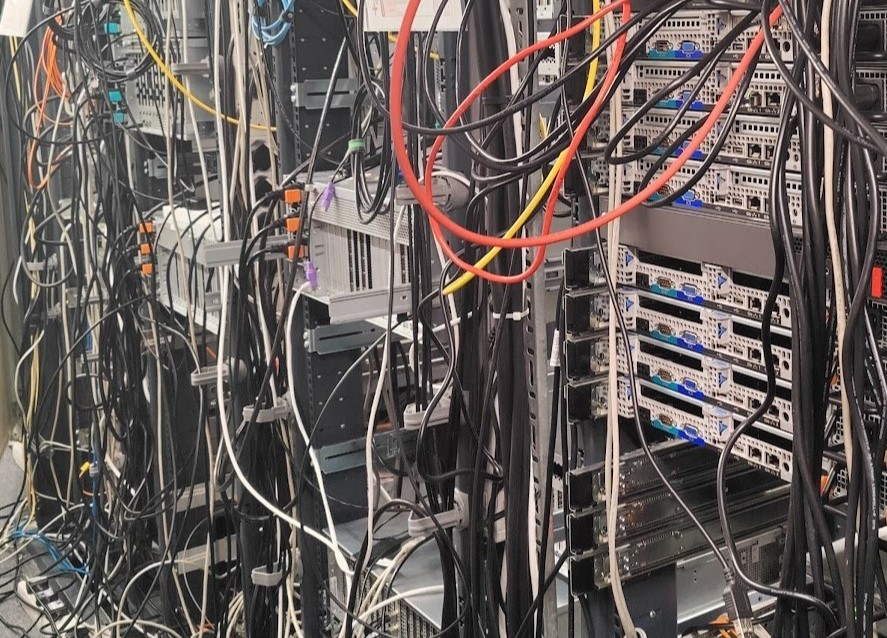
\includegraphics[width=0.40\linewidth]{images/server_racks.jpg}
    \caption{Server Rack within the School of Computer Science\cite{server_pic}}
    \label{fig:server_rack}
\end{figure}

This is another reason that typical data centre infrastructure management software (DCIM) solutions cannot usually apply to these spaces, they are often designed for large data centres, where laptops can be used easily. For example, see below a photograph of the ideal system administrator setup (Fig. \ref{fig:ideal_server_setup}). Where there is enough space to navigate between racks with a cart. In many scenarios, like that at Nottingham, this isn't an option. A tool that can be used on a mobile device in these less-than-ideal conditions has been something worthy of investigation. As mentioned the server space in Fig. \ref{fig:server_rack} is a good example. Before upgrades, the space was poorly lit and still is relatively cramped. It`s not particularly feasible to use a laptop in this space comfortably. But, as most alternative solutions assume the opposite and have cluttered user interfaces (UI), it makes certain tasks more difficult. The app provides a simplified, yet comprehensive interface to replace the need for a laptop in these situations.

Further, the layout of servers and hardware shown above, made tracking cables completely impracticable and a mobile application has proved to be a great aid in the solution to this problem. Being able to see the configuration of a server visually, in situ, has shown prospects to be a great aid in the refactoring of the server space.

\begin{figure}[H]
    \centering
    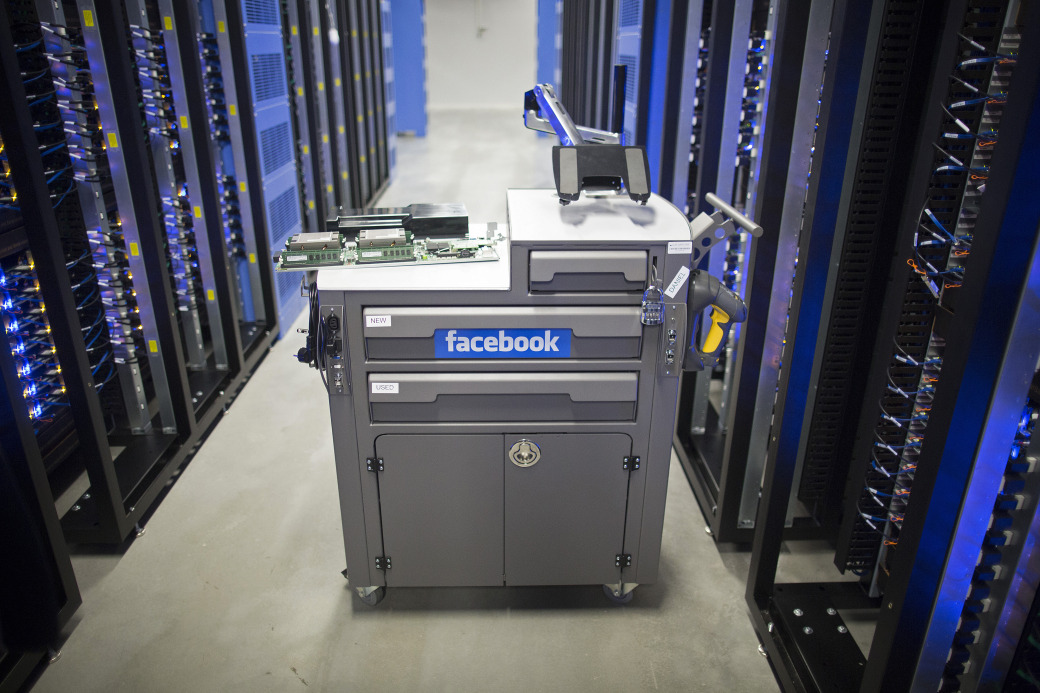
\includegraphics[width=0.40\linewidth]{images/facebook_cart.jpg}
    \caption{A more ideal administrator setup \cite{rosenblatt_2018}}
    \label{fig:ideal_server_setup}
\end{figure}

Comparatively, shown below is another server space at Nottingham, which is focused on networking infrastructure. This shows a more realistic, ideal setup for what is can be achieved outside of data centres (\ref{fig:ideal_server_space}). Whilst the space is still cramped, the cable management is better and so the tracking of cables is more straightforward. Whilst this makes the task of tracing cables easier, it doesn't make the task of understanding the configuration of the server any different. This is where software like Netbox provides a source of knowledge that contains more information than a cable label can. But, critically the server space is still cramped and the use of a laptop is still impractical. Therefore, the use of a mobile application is still a great aid in this situation.

\begin{figure}[H]
    \centering
    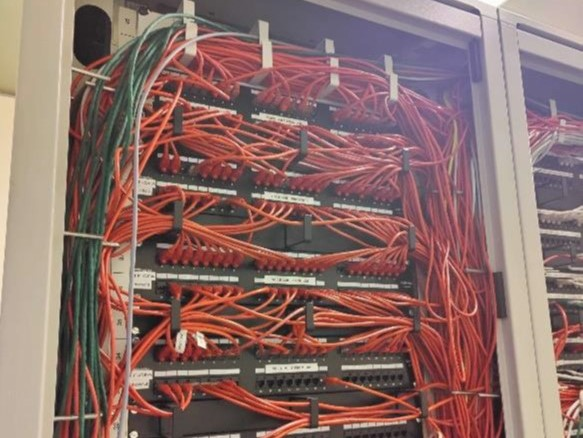
\includegraphics[width=0.36\linewidth]{images/server_racks_clean.jpg}
    \caption{More ideal and realistic server space\cite{ideal_server_pic}}
    \label{fig:ideal_server_space}
\end{figure}


\subsection{Aims \& Objectives}
\label{sec:objectives}
The project's aims with their respective objectives.
\begin{enumerate}[noitemsep, labelindent=0pt, label=\textbf{A\arabic*}]
    
    \item To create a tool that will allow for cable configuration of server hardware to be
    easily digitised, visualised, queried and updated. 
        
    \begin{itemize}[noitemsep, topsep=0pt]
    \item To achieve this, the tool will be integrated with Netbox, an open-source DCIM software for managing and maintaining network infrastructure. This will act as the backing database for the tool and will allow for the tool to be used in a wider context of server management.

    \item The tool will use Netbox's API to query and update the database whilst using intuitive UI to allow for easy use.
        
    \item To achieve visualisations, the tool will illustrate the cable connections between devices, showing data clearly and concisely.
    \end{itemize}
    \item To create an in situ cross-platform mobile app that can be utilised in restricted
    spaces.    
    \begin{itemize}[noitemsep, topsep=0pt]
        \item To achieve this, the tool will be cross-platform and will be able to be used on any mobile device supported by the Flutter framework.
        \item The tool will be designed with a focus on Human-Computer Interaction, to ensure that the tool is easy to use and can be understood by a wide range of users.
    \end{itemize} 

    \item To create an app that can interact with other open-source software easily
    \begin{itemize}[noitemsep, topsep=0pt]
        \item The tool will be open source, so modifications can be made to the tool to allow for it to be used in other contexts.
        \item The tool will be built around modifiable models that can be changed easily for other software or a custom build backend.        
    \end{itemize}
        

\end{enumerate}

\subsection{Background}
\label{sec:background}
During my work for the Research Support Team over the last 18 months and the challenges faced with server administration, I came to realise that there was a missing tool that could make a lot of tedious and time-consuming tasks easier. Once I began researching solutions to these problems, I came across Netbox, which is now our `source of truth' for our server space. It contains information about all of the hardware in the space, including the cables that connect them. Once Netbox began filling with data, the problem of finding and modifying that data in situ arose. I found that using the full-size interface was too clunky and so I wondered if there was a mobile app alternative, but there wasn't. This was the initial inspiration for the project. I wanted to create a tool that could be used in situ, on a mobile device, to make the task of managing the server space easier. Whilst it can be appreciated that in large data centre applications, a mobile application like Keeptrack (developed in this project) might not have the same desirability as a desktop application. But, acting as a companion tool alongside the desktop open-source software could be a great aid. With benefits for both platforms, they can be used in different situations, making workloads simpler and more efficient. Whilst there exists a companion app for a paid-for DCIM solution, there is no open-source equivalent. This was a gap in the market that the project aimed to fill, as well as carrying out research into the usage of mobile applications in this context.

\pagebreak

\section{Related Work}

In this section, three aspects of related work are discussed; existing applications similar to the project, related human-computer interaction research, and finally, papers related to the technical aspects of the project.

\subsection{Related Products}
\label{sec:app_reviews}

Following research on open-source and paid-for cable management/DCIM software, it was found there are limited options that have access to the trial versions without a legitimate business interest. This restricted the options of related applications that could be investigated. This aside, there follows three different software packages that are relevant to the project. Including; Sunbird DCIM\cite{Sunbird}, a paid-for solution with a trial accessible publicly. Next, Pathfinder Mobile \cite{Pathfinder}, a mobile counterpart to the enterprise `Pathfinder' package, was the only high-quality mobile solution that was discovered. Finally, Netbox \cite{Netbox}, the open-source DCIM software that the project has been built around. These three packages were shown to three individuals within the Research Support Team and their feedback was recorded.

\subsubsection{Sunbird DCIM}
\label{sec:sunbird}
Sunbird DCIM is a feature-full DCIM Package with a significant list of components. Their client list includes Paddypower, Betfair, eBay \& COMCAST \cite{Sunbird-we-know-data-centres}. When trialling dcTrack, their DCIM software, the immediate impression is that it is feature-rich, including monitoring environment, security, cooling as well as having asset and connectivity tracking. Whilst the server spaces within Computer science at UoN could benefit from a tool like this, its implementation and management would be quite the task. The tool is designed for large data centres and would be overkill for the server spaces within the school and other SMEs. For example, in fig \ref{fig:sunbird_dcTrack}, the space shown is approx 10x larger than that at Computer Science and this is one room in the example. 

\begin{figure}[H]
    \centering
    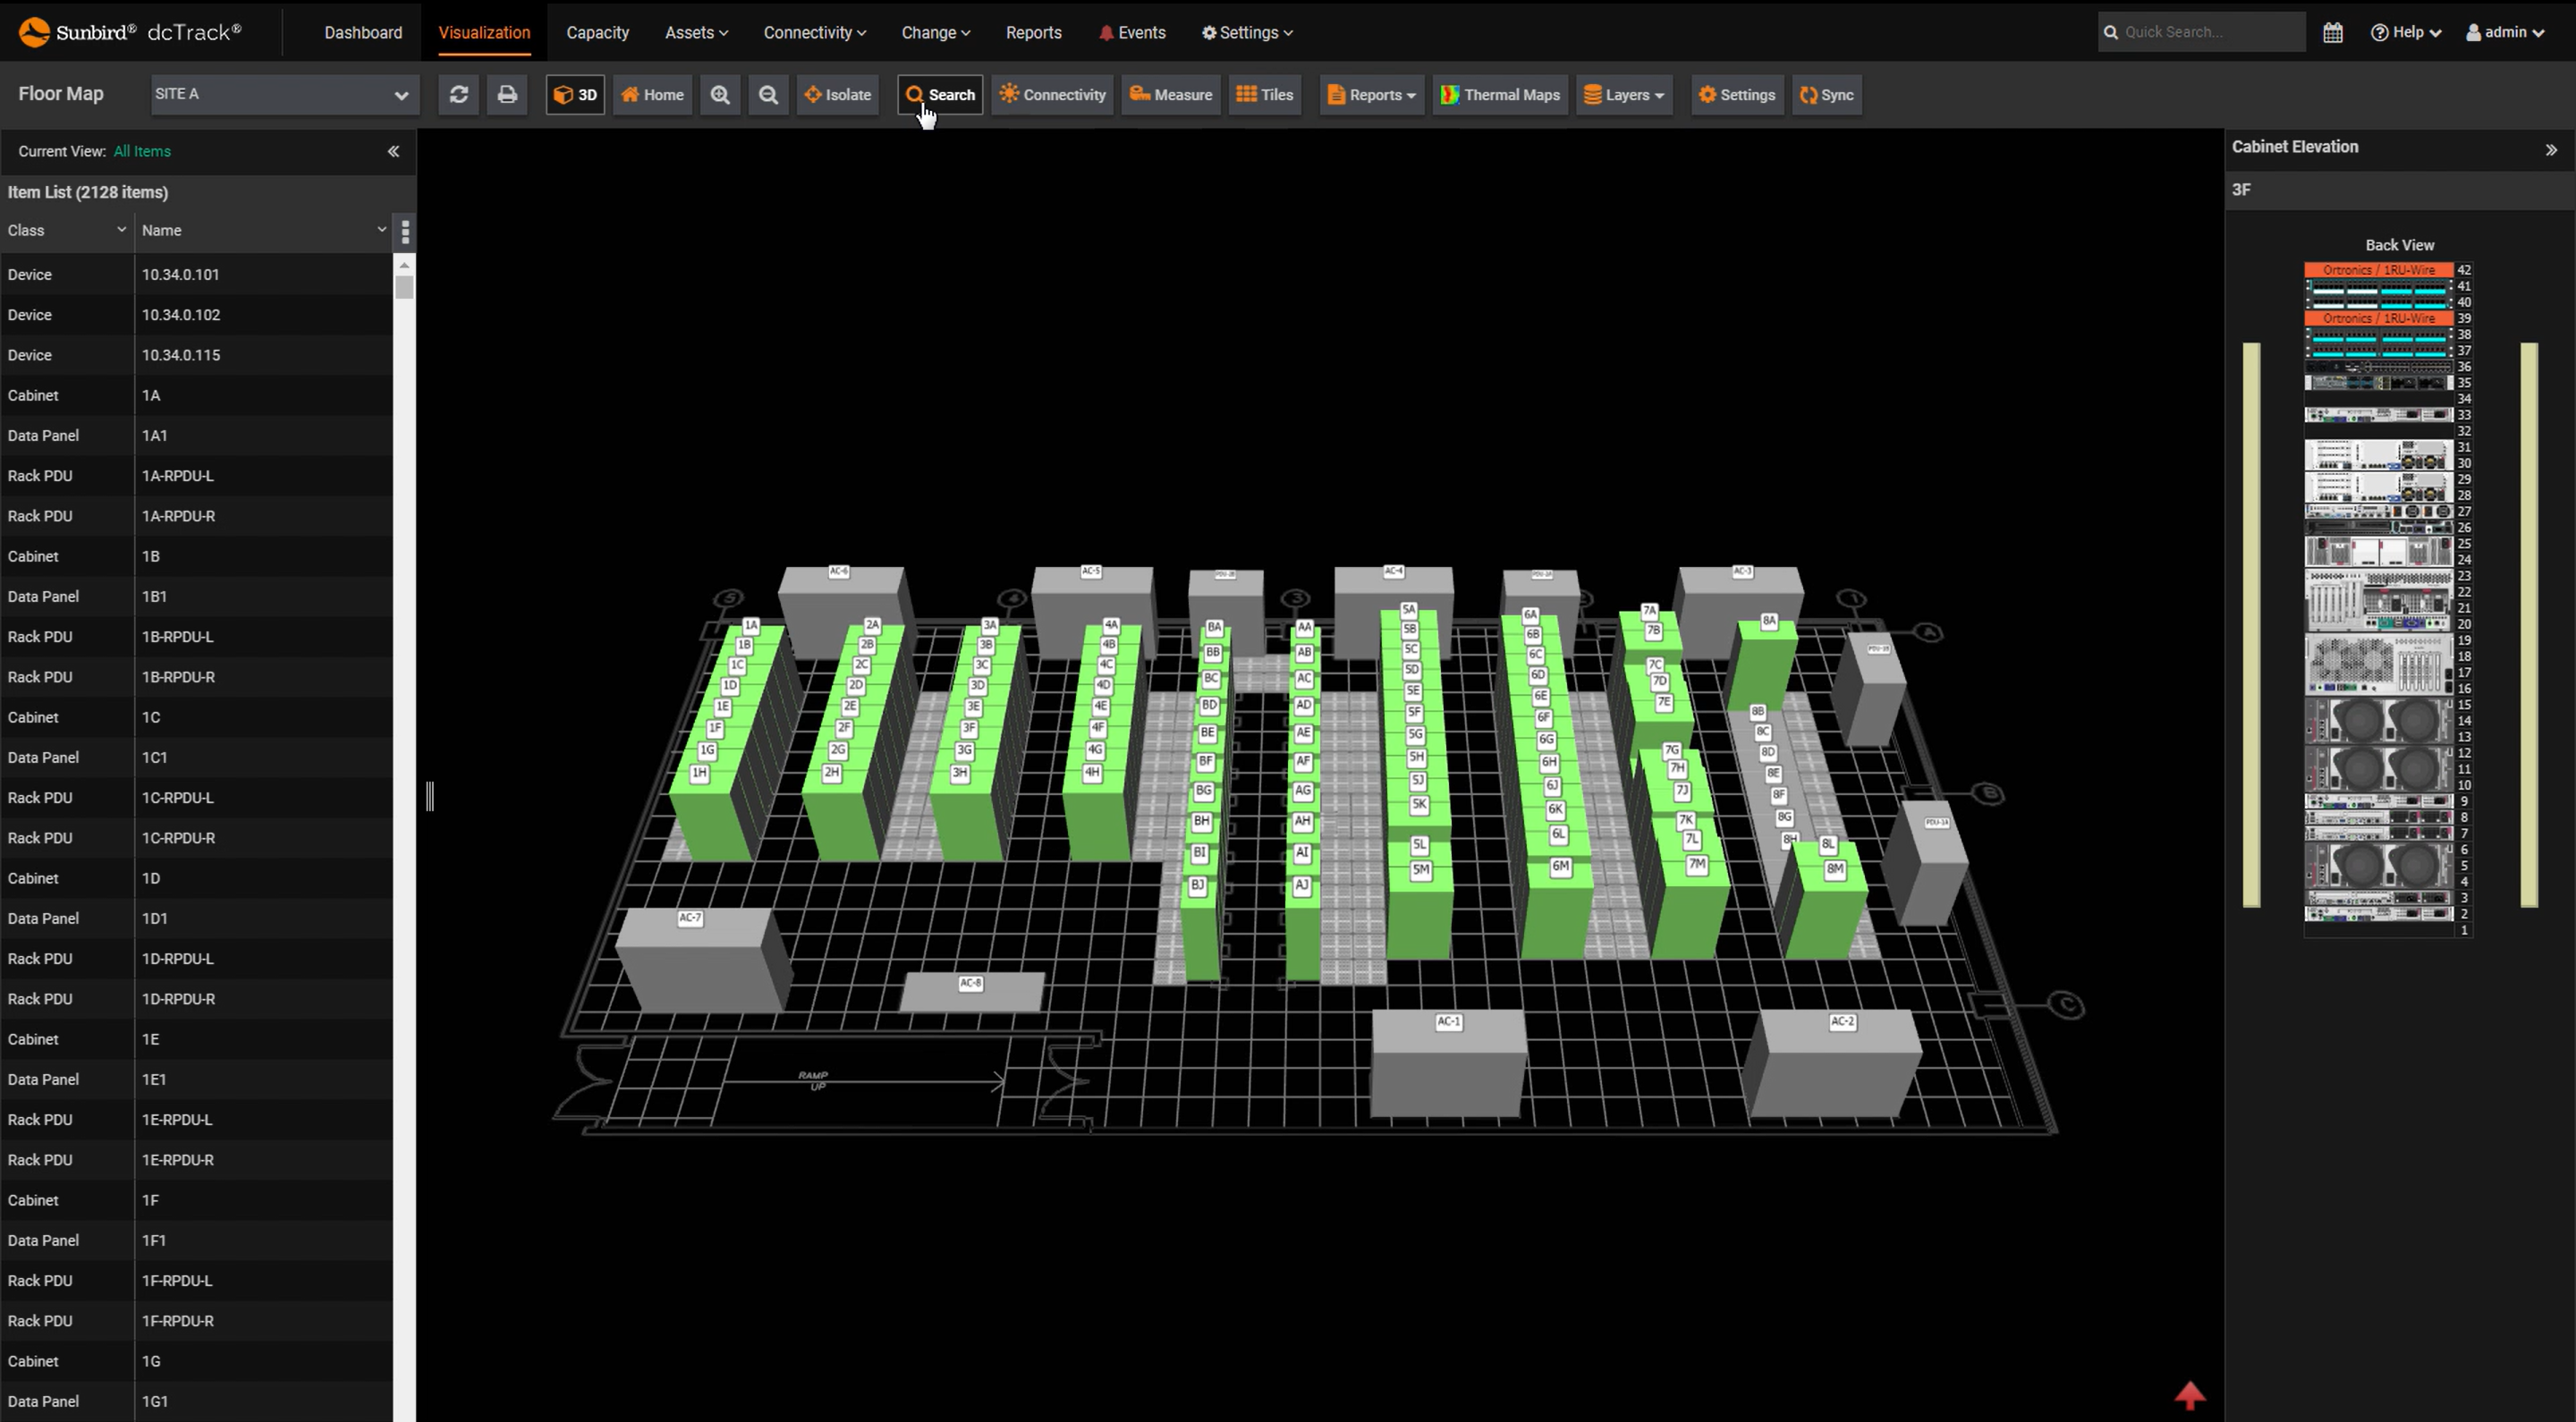
\includegraphics[width=0.7\linewidth]{images/sunbirddcim.png}
    \caption{Sunbird DCIM - dcTrack}
    \label{fig:sunbird_dcTrack}
\end{figure}

Though, some of its features could be useful in the implementation of the project. For example, the visualisation of data centres via a 3D model could be an interesting feature to implement in the project but might be out of scope. Especially with the additional research and testing that it would require. On the other hand, the search for assets and connections that Sunbird has, while thorough, is not as intuitive as the project aims to be. The immediate view lists all assets and their information, with 25 columns of data. It is overwhelming and not very useful without filters and custom views. Further, Sunbird intends to serve clients that might have thousands of assets, not quite hundreds like Computer Science has, so the requirements of searching and filtering are different. Though, filtering by an extensive set of categories is a useful feature and could be implemented in the project, but more intuitive. 

Sunbird is a prime example of what the project is not. It is enterprise-level DCIM software that is `overkill' for SMEs. Whilst it is a great tool for large data centres, its depth of features and complexity would add to the difficulty of implementing and using the software day to day.

\subsubsection{Pathfinder Mobile}
\label{sec:pathfinder}

Pathfinder Mobile is a mobile component to the complete Pathfinder package, it is designed to be used in conjunction with the full software and used as an `anytime and anywhere' \cite{PathfinderMobile} tool. It allows existing users of Pathfinder to access data remotely and in situ, with an intriguing focus on `work orders'. These work orders are created at a workstation, i.e. a laptop, which then synchronizes the work orders with the mobile app. From here the work orders can be executed on-site by using `graphical instructions support'\cite{Pathfinder}. Finally, on completion, all changes are uploaded to the Pathfinder client. See below for screenshots from the Pathfinder Mobile app. 

\begin{figure}[H]
    \centering
    \subfloat[\centering Side Panel]{{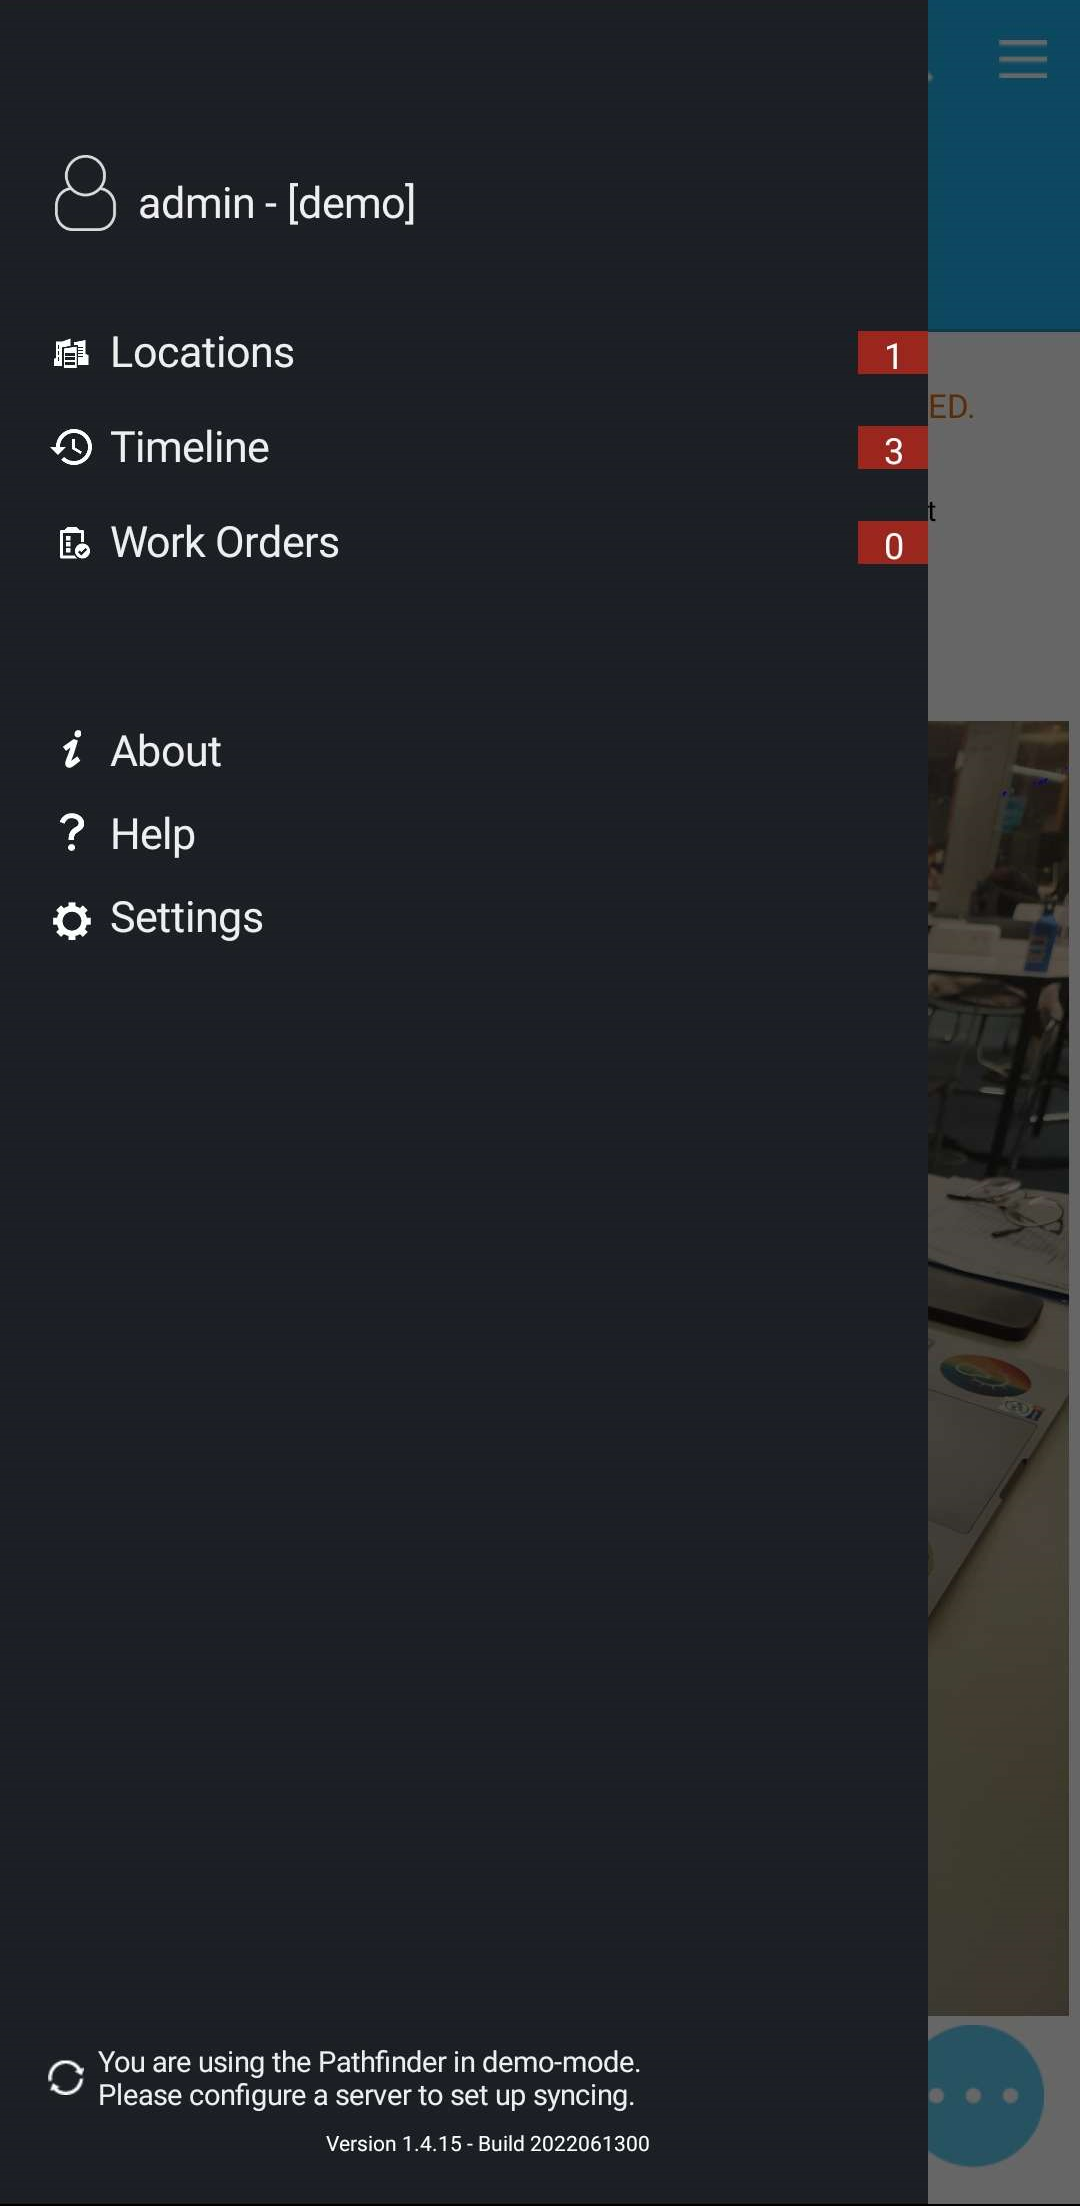
\includegraphics[width=4cm]{images/pathfinder_overview.png} }}
    \qquad
    \subfloat[\centering Network Trace]{{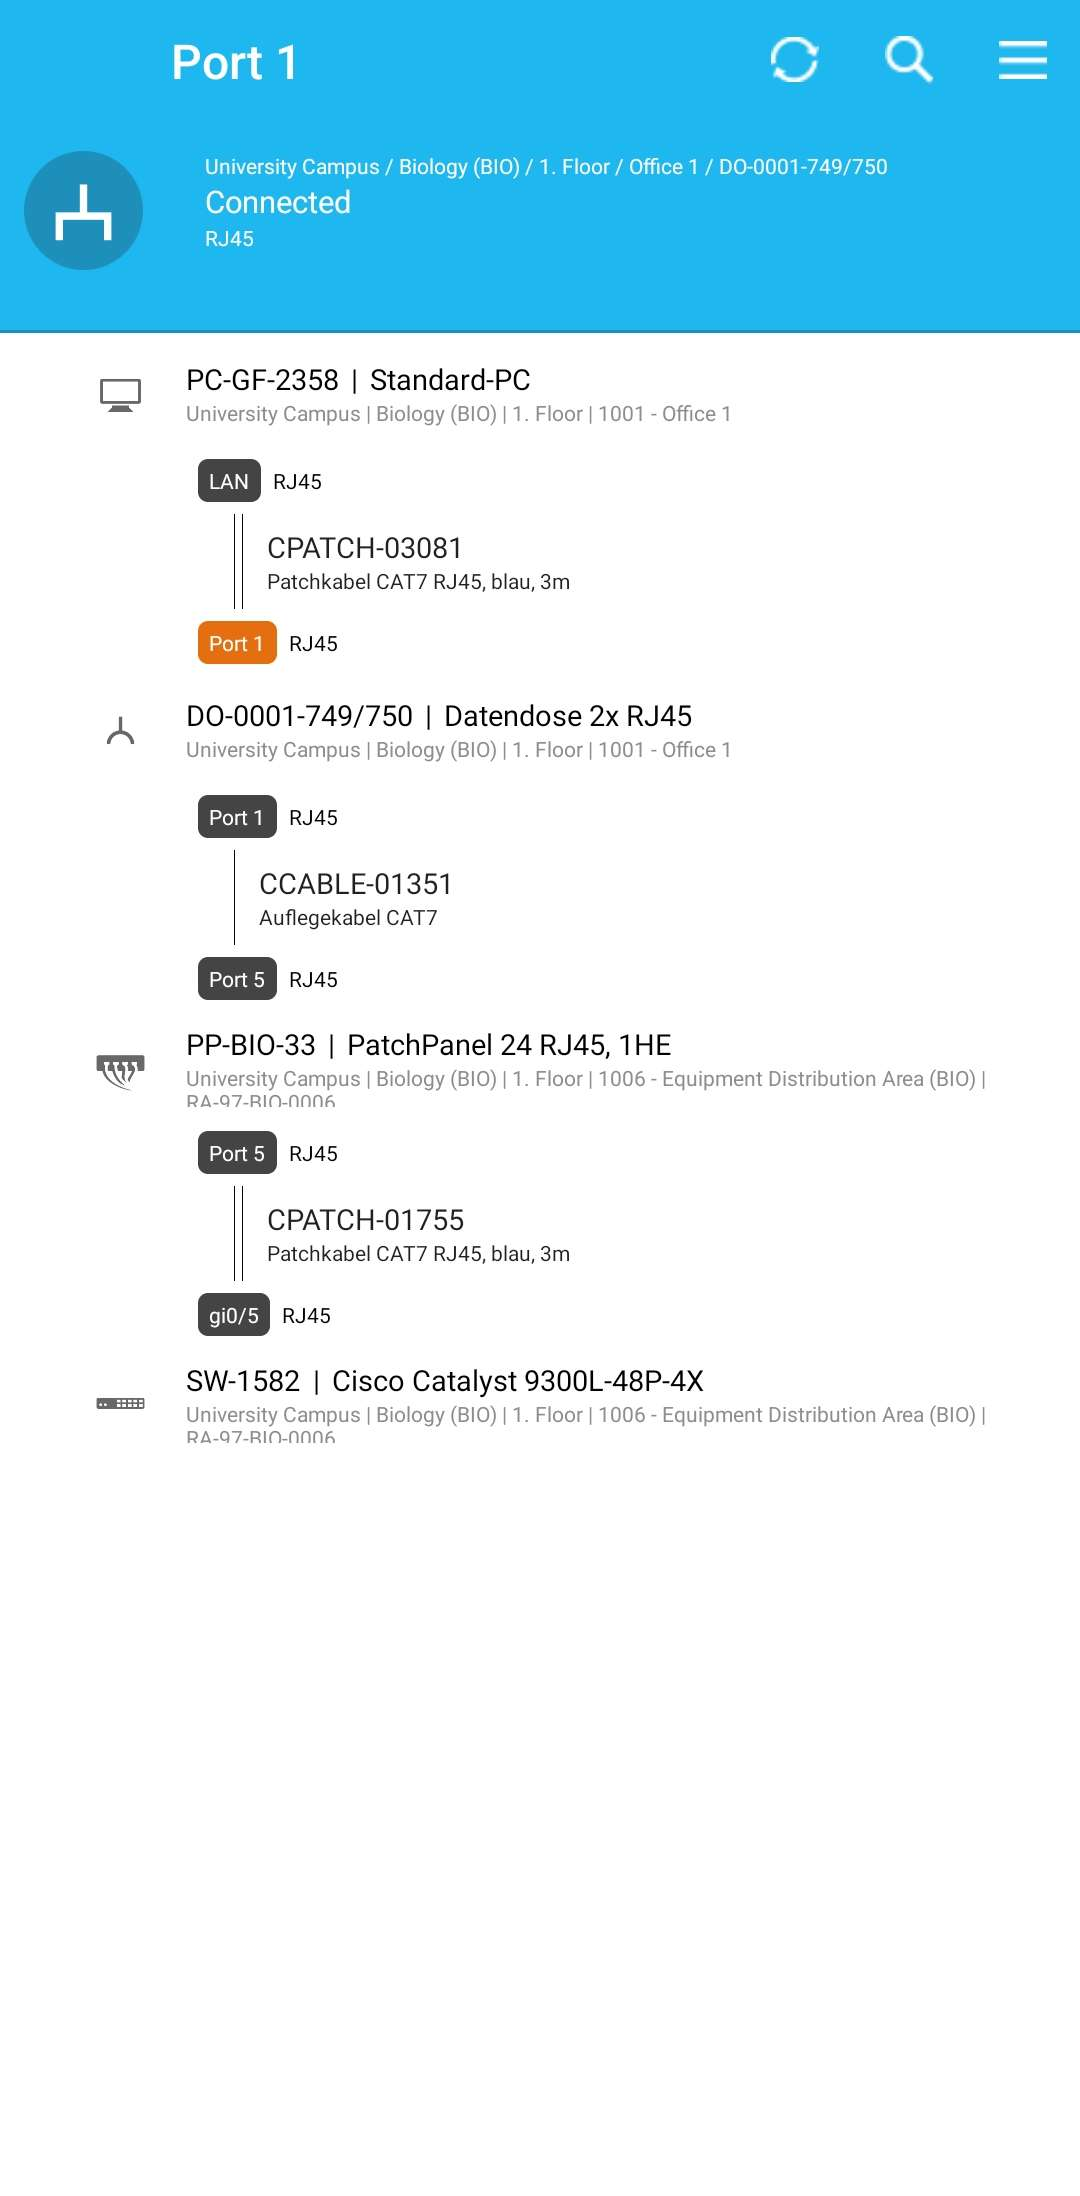
\includegraphics[width=4cm]{images/pathfinder_trace.png} }}
    \caption{Screenshots of the Pathfinder Mobile App}
    \label{fig:pathfinder_screenshots}
\end{figure}

A similar environment interaction would work well for this project, with more complex modifications being completed/generated on a desktop client on the school's Netbox instance, i.e. templating. Then once completed, this can be synchronized with the mobile app to be used in situ. For example, verifying the correct cable is connected to the correct port. Additionally, completing work that is easier on desktop (due to say, more typing) and then synchronizing it to the mobile app so that in-situ modifications can be done easier. For example, adding an asset and then adding its networking information.  

The Pathfinder app also allows for quick access to networking information, where users can complete the tracing of connections. Whilst this already was a core intention of the project, Pathfinders' method to visualise this is intuitive and similar to that which was discussed in the first current state analysis interview. These interviews are discussed more in detail in section \ref{sec:current_state_analysis}, but, notably, an interviewee mentioned a good method to do a visualisation is to list devices in a scrollable view. Then each connection between them is drawn on the screen, along with device and interface information displayed as well. This is also similar to the method used by Pathfinder, with device name, location, interface name, type and cable type being displayed. This would aid in easing the process of tracing cables and connections, as well as verifying that the correct cable is connected to the correct port.

One aspect of Pathfinder that could be improved upon is the search functionality to find assets. Whilst they describe their search as being `text-rich'. It seems to be less intuitive, and does a search based on every field, meaning that results for a simple search can be overwhelming. This is something that the project aims to improve upon, with a more practical search method, separating searches based on possible results. For example, not returning cables or power supplies when the user is only looking for devices. Further, their search by barcode scanner only simply enters the code into the search bar, not necessarily a bad method, but not as intuitive as it could be, for example - a button to scan the barcode, that on completion, automatically displays the asset information rather than needing another step.

A notable design element that the Pathfinder app implements is the focus on locations, assets, and connections in a hierarchical sense. For example, one method of displaying the data is to have a list of locations, then a list of assets within that location, and then a list of connections between those assets and so on. This is something that the project has also implemented due to the feedback from the interviews and has provided a straightforward way to display sometimes complex data.

Overall, Pathfinders mobile app has been a good reference point for the project. It has a similar focus and a similar method of visualising data. Though it is a companion of a larger software package that exceeds the current requirements of the school, it has features that have been referred to and implemented in the project.  

\pagebreak

\subsubsection{Netbox}
\label{sec:netbox}
Whilst searching for a DCIM solution for the School of Computer Science, Netbox became a clear choice. It has a solid feature core, it's open source, self 'hostable' and could help solve the problems that the school faced. As discovered during the Current State Analysis and personal experiences, the server rooms within CS are documented poorly due to a lack of consistent historical data. Most of the information is stored in the memory of long-gone staff or out-of-date spreadsheets. Netbox is to act as a `source of truth'\cite{Netbox}. More information on Netbox is included in the implementation section \ref{sec:development}. 

Netbox is built upon several data models, which interact and are nestable with each other. For example, a device can be a child of a rack, which is a child of a site. This is a similar method to Pathfinder and allows for a deeper relationship between data. This parent, child relationship allows for efficient tracing between devices and connections. With this approach and the solid API that Netbox provides it is possible to fetch this data and display it in a way that is intuitive and easy to use. 

One drawback of Netbox is the tracing of connections and the addition of cables. It seems that the relationships can get a bit lost, and it is not as intuitive as it could be. This is something that the project improves upon, especially with in situ tracing, where navigating a large screen interface can be difficult. A primary example of this is the multiple types of ports or interfaces that a device can have. For example, a switch can have console ports, power ports,  network ports, and management ports; all of which are displayed on different pages and can be nested within each other. It can be difficult to navigate this, especially when the device has a lot of ports. This is something that the project aimed to improve upon, with a more intuitive and efficient way to display this data.

Whilst Netbox is a great tool, it is not without its flaws. This project solves one of its main issues, the clunky in situ use experience of the interface. Whilst it has a mobile-friendly web interface, there are limits as to how friendly it can be. The limited screen retail needs to be used efficiently, and having a complex interface nested inside a browser app is not the best way to do this. Additionally, there is a lot of data to be loaded and displayed, in a browser this can show as loading bars and a low frame rate. Here is where Keeptrack comes in, to sit on top of Netbox and provide a more intuitive and efficient interface for the user.  


\subsection{HCI and User Experience}
\label{sec:HCI}
There is a lack of significant research into areas of Human-Computer Interaction (HCI) and User Experience in the context of server management. But for the few relevant papers, they have aided in the development of the project. The first paper is a write-up by Yin et al. \cite{cloud3dview} regarding their demonstration of Cloud3DView at SIGCOMM '13. Cloud3DView is an interactive 3D visualisation tool used for cloud-focused data centres. It uses FPS gamification to allow users to monitor situations and visualise data from a user-friendly interface, all remotely. Cloud3DView also included a focus on its use of `cutting-edge HCI technologies' \cite{cloud3dview}. Whilst the paper itself doesn't go into the reasoning of why certain HCI choices were made, it shows a good example of how a mobile device can be used to interact with a data centre and can be used to improve efficiency and user experience. 

Though the focus of this project isn't to be a 3D visualisation tool, one aspect of Cloud3DView is the ability to view data about the devices in a 3D environment. Whilst, a 3D visualisation is out of scope for Keeptrack, an augmented reality feature was considered to be implemented and was discussed in the Current State Analysis interviews. This feature would allow users to view data/connections concerning the devices via a camera on their mobile device, offering an alternative method of visualisation. Though to add this, significant research would need to be done into the best way to implement this feature and how it would interact with the server room environment.

Notably, in the paper about Cloud3DView, there was a focus on using mobile devices to be used for data visualisation, but no mention of their possible use for data entry. With the nature of the data being entered in server management, in some cases, a mobile format may offer a more intuitive/accessible platform than a desktop device. For example, entering the connection between two assets, where the information can be verified in situ in real time versus sitting at a desk far away. This is one of the workflows that the project was developed to improve upon.

An important benefit of using mobile devices for data entry is the ability to use multiple interface types to enter data. For example, a user can enter data via an alphanumeric keyboard, numerical keypad, calendar picker, lists etc all whilst benefiting from the ease of a touchscreen interface. A comparative analysis into different data entry design patterns investigated three different patterns for seven different data types for a set of nine tasks testing different patterns \cite{myka2019comparative}. The investigation completed a set of usability tests to determine which pattern was the most effective, with different patterns benefiting different tasks/data types better than others. The results from this study have been used to inform the design of the interface for the project. Specifically for this project, the most relevant data types are; small numbers, single-choice lists and text.

On a similar note, a study into the structure of data entry on mobile devices noted that existing interfaces `interfere with user input' and force `complex interactions to enter simple information' \cite{van2007gui}. This is especially apparent in some cases of the Netbox interface e.g., as mentioned previously, adding cable connections. Whilst, naturally, there are limitations as to how streamlined an interface can be on a desktop-based web application, there is more room for improvement on a mobile application. For example, the addition of a cable on mobile can be reduced to far fewer steps than on the web interface. Whilst it might reduce the granularity of the data, it would be a trade-off that would be worth it for the ease of use. Additionally, the project aimed to improve upon the current interface, not replace it. The current interface is, in theory, still available for users who prefer it, or for more complex tasks.

Kleek et al's \cite{van2007gui} study further focused on the structure of data entry on mobile devices, its importance, but also the importance of not creating interfaces that deter users from entering data. Highlighting a fine balance between the two. One of the sources of problems for the school is the lack of data ever being entered anywhere. If the project has an interface that dissuades users or is perceived as too tedious then it will not solve a key problem. This project took upon the findings of this study to ensure that the interface is intuitive and easy to use. For example, an automatic filtering search bar for assets and replacing text fields with barcode scanners or other input methods.

\subsection{Asset Identification \& Visualisation}
\label{sec:technical}

One key part that the project aimed to improve is the searchability of assets, i.e. finding the asset desired quickly and accurately through many means. The current method of asset identification is inconsistent with different naming conventions, ID codes, labels, no labels, hostnames etc. The Centre for the Protection of National Infrastructure (CPNI) produced a paper on the importance of asset management, specifying that, `all organisational assets and systems that are necessary for the delivery of effective operations or are of specific organisational value, should be identified.'\cite{cpni}.

Not only is it important to identify assets whilst they are in use, but also for documenting any changes, journal entries, ownership, location etc. This project also aimed to improve upon this, with a focus on the identification of assets being homogenous and consistent. Keeptrack uses the Netbox model IDs as unique identifiers for each asset, cable and interface. This way, they can be referred to individually and updated consistently. 

In this project, assets are considered to be physical server hardware, such as servers, switches, KVM`s, NAT etc. but also cabling, such as ethernet, fibre, SFP and power. To identify each of these assets uniquely it was decided that an encoded label would be best. A comparative study into barcodes, QR-codes and RFID systems in the library environment looked into the respective advantages and disadvantages of each \cite{lotlikar2013comparative}. Going by these attributes, it is more sensible to use Barcodes or QR codes for the project. RFID tags are more expensive, as well as have a higher risk of tag collisions. This occurs when many tags are in close proximity\cite{lotlikar2013comparative}, like that of a server room, and a reader misreads their value to be another. An issue like this would likely add to the time-consuming tasks and make for a more frustrating workflow. Further, a specialised reader is likely needed and so another handheld device would need to accompany the app. Additionally, a paper written on the review of QR codes highlights that QR codes can store more data in the same area, have data redundancy, are faster to scan and are `readable from any direction in 360\degree'\cite{mishra2017review}. Whilst these benefits seem to make it the clear choice over barcodes, QR codes contain data in both dimensions. Though this is a benefit in most use cases, it is likely to pose a problem when scanning codes stuck to ethernet cables.

Where, barcodes contain data in one dimension which is then repeated vertically, allowing for their placement to be more dynamic, e.g. on a cable. This is clearly shown in Figure 3 of Mishra et al., fig. \ref{fig:barcode}. So, for this project, it was initially decided that it will use barcodes for cables, and then QR codes for other assets will be used. But after the interview processes and observations, it was decided that QR codes would be more beneficial as they can store more contextual data. It was realised following consultation with CGI, the global IT consulting firm, that having labels that only hold abstract data can be considered a single point of failure to gather information. Especially as it was initially decided that the information stored for cables will be a random short number assigned to each cable, suitable for barcodes - But completely abstract for humans to read. So in the situation of Netbox being inaccessible, or the QR code is damaged, the information stored on the label would be useless. Therefore a combination of a meaningful label and a QR code would be used. Each QR code can then store the Netbox unique ID for that cable. This way, the QR code can be scanned and the information can be retrieved from Netbox via the URL directly. This is a more robust system than just having a label with a randomly generated number. Additionally, storing the URL means that any device with QR-capable scanning  will be able to be redirected to Netbox and the cable directly.

\begin{figure}[H]
\centering
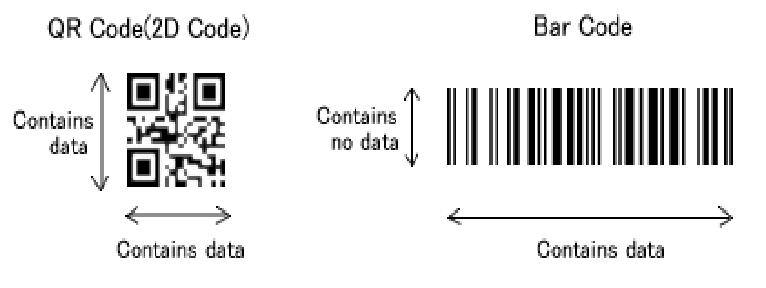
\includegraphics[width=.50\textwidth]{images/barcode_mishra.png}
\caption{Barcode vs QR code}
\label{fig:barcode}
\end{figure}

Whilst the addition of the augmented reality visualisation stretch goal was dependent on time and the success of other elements. It was still important to consider related work with these features, especially as it could be a feature added on with future development. At the same time, already investigating Cloud3DView \cite{cloud3dview}, which uses 3D visualisation, a more apt implementation would be by using the QR codes placed on assets to aid in visualising data. This is very similar to the work outlined in the paper, `Applying QR code in augmented reality applications' \cite{applyingQR}. This paper displays how the elements of the QR code can be used to position elements in the AR scene and simultaneously generate information embedded in the QR code. Should this be a feature that can be implemented in the future, it is likely the best approach will be to follow a similar method as to what Kan et al. set out \cite{applyingQR}. Further, there already exists a cross-platform plugin for Augmented Reality in Flutter which can be utilised \cite{ar_flutter}, this would be a good starting point for future development. This feature would allow the user to scan the environment with the device's camera and see the assets in the room, as well as the cables connecting them as they walk around. Possibly allowing the user to see the cables in the room and their traces to find ports, locations etc. This would be a very useful feature for the user to have, as it would allow for a more intuitive and interactive way to visualise the data and the task of tracing connections. Though, the amount of time it would take to implement this feature would be significant, especially with the need to 3D map the server room as well significant development of a backend system to store the data.

\section{Description of the Work}
\label{sec:work}
This project aimed to create a mobile application that will allow users to add, view and manage assets and cables in server rooms. With the specific application to Small/Medium enterprises. The application has been built using Flutter, a cross-platform framework which will allow for the app to be used on both Android and iOS devices, but also has support for Windows, Web, Mac and Linux ecosystems. The application has been built upon the Netbox DCIM software \cite{Netbox} and their RESTful API \cite{NetboxAPI}. This API allows the app to communicate with the Netbox database as well as provide a mobile functionality of Netbox's interface.  

The project has built upon the API to create a more user-friendly and intuitive interface for server administrators to use. With this in mind, a second key aspect was to investigate the best interface for data entry in this context. This was done by interviewing and observing the system administrators at the school using iterative prototypes of increasing fidelity. This gave the project a human centred design approach, allowing for the app to be tailored to the needs of the users.

\subsection{Project Scope}
\label{sec:stretchgoals}

Following the interviews during the current state analysis and the investigation of similar work, I considered a range of methods to tackle the project. One of the most aspirational goals was to implement the augmented reality visualisation feature. This feature would allow users to visualise asset information and networking details in a highly interactive way. Due to the time constraints of the project, it wasn't something that was feasible for its time scale and it was deemed to be out of scope. 

Below is an outline of the features that were considered to be out of scope for the project. Though, it is important to note that these features are not considered to be impossible to implement, but rather that they would require significant development time and would be out of scope for the project.

\begin{itemize}
\item Journaling for assets, allowing for notes to be added to assets, e.g. when a new component is added, or when a component is removed.
\begin{itemize}
    \item Originally it was intended to use the existing journaling feature in Netbox, but as of the time of writing this report, this feature did not a good exposure via the API and so would require significant development outside of the core focus. Though it is something that could easily be added.
\end{itemize} 

\item Auditing of assets, allowing for the user to scan an asset and then be presented with a form to fill out, e.g. the asset is in good condition, or the asset is faulty. 
\begin{itemize}
    \item Similarly to the above, it was intended to use the journaling feature to add this functionality but given the limited API exposure, it was also deemed to be difficult to implement. Though, it was not considered at the time of implementation to utilise the ability to comment on a device and could have been investigated with more time. 
\end{itemize} 

\item In-App SSH terminal, allowing for the user to connect to a device and run commands, e.g. to check the status of a service. 
\begin{itemize}
    \item Whilst this was a great idea in the conceptualization of the project, a considerable oversight was the networking restrictions that would restrict this feature drastically. In the case of computer science and their current infrastructure, most server devices are under separate virtual LANs (VLANs). These VLANs don't have wireless capabilities and so a mobile device would not be able to connect. Whilst in other scenarios, this might be less of an issue and is a good concept to implement for quick testing/diagnosing. 
\end{itemize} 

\end{itemize}

\pagebreak

\subsection{Functional Specification}
\label{sec:func_spec}
Below is the functional specification of the software outlying what the application will do.
\subsubsection{Authentication and Security}
\label{sec:spec_auth}
\begin{enumerate}[label={\fbox{AUTH\_SPEC\_\arabic*}}, leftmargin=*, labelindent=\parindent]
    \item The app will utilise the Netbox API to provide authentication and a secure connection to the Netbox database.  \label{spec_auth_1}
    \item The app must use the user's username and password to authenticate with the Netbox API to create a token. \label{spec_auth_2}
    \item The app must detect if a user is logged in and if not, prompt the user to log in. \label{spec_auth_3}
    \item The app must know if the token being used has expired and then prompt the user to log in again. \label{spec_auth_4}
    \item The app must not display any data if the user is not logged in or if the token has expired. \label{spec_auth_5}
    \item The app must allow the user to log out of the app and delete the token automatically. \label{spec_auth_6}
    \item The app must store the token securely on the device. \label{spec_auth_7}
\end{enumerate}

\subsubsection{Asset Management and Information}
\label{sec:spec_asset}
\begin{enumerate}[label={\fbox{ASST\_SPEC\_\arabic*}}, leftmargin=*, labelindent=\parindent]
    \item The app will allow the user to view and manage assets and cables in the Netbox database. \label{spec_asset_1}
    \item The app shall allow the user to add, edit and delete cables in the Netbox database. \label{spec_asset_2}
    \item The app shall allow the user to search for assets in the Netbox database. \label{spec_asset_3}
    \item The app must be cross-platform and support Android and iOS devices. \label{spec_asset_4}
    \item The app must be able to scan QR codes and barcodes.  \label{spec_asset_5}
    \item The app must be able to visualise cable connections. \label{spec_asset_6}
    \item The app must allow users to search for connections and assets via a hierarchical search. \label{spec_asset_7}
\end{enumerate}

\subsubsection{User Interface}
\label{sec:spec_ui}
\begin{enumerate}[label={\fbox{INTF\_SPEC\_\arabic*}}, leftmargin=*, labelindent=\parindent]
    \item The app must use highly contrasting colours to ensure good accessibility. \label{spec_ui_1}
    \item The app should have a dark and light mode to allow for user preference. \label{spec_ui_2}
    \item The app should allow the user to toggle between the dark and light theme easily.  \label{spec_ui_3}
    \item The app should use Material3 widgets and icons for a consistent look and feel. \label{spec_ui_4}
    \item The app should use Material3 icons for increased usability and learnability. \label{spec_ui_5}
\end{enumerate}

\section{Methodology}
\label{sec:methodology}

With all of the aims and aspects of the projects in mind, it was decided to use a human-centred design approach, with iterative prototypes of increasing fidelity. This focus was decided based on the problem itself, and the complexity of what a solution would entail. Creating a good solution needed user involvement throughout and therefore this was deemed the best approach. Then, with user evaluation and feedback, the final product would then be created. The following list outlines, in order, the steps taken to complete the project.

\begin{enumerate}[noitemsep]
    \item Create low-fidelity prototypes
    \item Current state analysis and initial interviews
    \item Create higher fidelity interactive prototypes and gain user feedback.
    \item Minimal Viable Prototype with user feedback
    \item User observations and interviews.
    \item Create a final product with observation suggested changes.
\end{enumerate}

On top of these steps, there was a need to decide upon the platform to build the app. Whilst knowing the app needed to be cross-platform, Flutter become the obvious choice. Not only with previous experiences working with it but also with the fact it has become the most popular cross-platform framework \cite{JetBrainsFlutter} used. Further, with personal work in aiding the development of Labmonitor\cite{labmonitor}, there is a familiarity with the code scanning package that has also been used in this project\cite{barcodeScannerPlugin}.

The approach of the app development was to use the Agile methodology, with the use of a Kanban board to track the progress of the project. This was done by using Trello to create a board with the following columns: To-Do, Doing/Waiting and Issue. Then as tasks were moved from the backlog/created. An example of the Trello board can be seen in Appendix \ref{sec:trello_board}.

\pagebreak

With the iterative nature of the project, it was decided to use a combination of user interviews and observations to gain feedback on the app and its features. The initial interviews and state analysis were run as one-on-one interactive discussions with the system administrators (RST) to gain an understanding of the current state of the system. For more details see the Current State Analysis and Initial Interviews section (\ref{sec:current_state_analysis}). Simultaneously, the interviewees were also shown related products and asked to give their opinions on them. This allowed for a review of features and user interfaces intending to gain inspiration for the next iteration of prototypes. 

With this information and feedback, a set of high-fidelity prototypes were created. These were then shown to the interviewees in a less formal setting, allowing for a more natural discussion. This allowed for a faster, less fixed iterative design process where changes could be made quicker and more easily. This higher fidelity prototype then slowly progressed into a minimal viable product (MVP). Then as development continued and the MVP was created, the user feedback was then used to make changes to the app. Once the MVP was completed, it was then shown to the interviewees again, this time for a set of user observations and discussions. 

From these observations and comments from the interviewees, the final product was then created by developing the existing prototype. This was primarily making slight changes to the user interface and adding small features that were requested. This process is outlined in more detail in the following sections.

\subsection{Current State Analysis and Initial Interviews}
\label{sec:current_state_analysis}

To begin with, using personal experience, knowledge and understanding of the requirements, a set of low-fidelity prototypes was made. These were primarily created to establish an initial set of features. A set of interviews were then conducted with the system administrators (RST) to extend upon original experiences.  Within these interviews, the current state of the system was discussed, to understand the current workflow and the problems that are faced from their perspective.

This was done by asking broad questions such as:

\begin{itemize}
    \item What are your opinions on the current state of the server room?
    \item What do you think could be improved?
    \item Do you have any suggestions for the new system?
\end{itemize}

Each interviewee was then shown the low-fidelity prototype of the application, intending to gather initial thoughts on the proposed layouts and to see if there were any features that they would like to see added/removed. Their responses were recorded and then analysed, to identify any repeating ideas, primarily using thematic analysis \cite{thematicAnal}. For more details on the analysis of the interviews and the points that were raised, see the interview analysis section (\ref{sec:ui_design_interview_analysis}).

\subsection{High Fidelity Prototypes}
\label{sec:high_fidelity_prototypes}
Once the initial interviews were conducted, a higher-fidelity prototype was created. This was done using Figma to create a set of interactive prototypes. Additionally, the theme of the app was generated using the Material3 Theme Builder for figma\cite{material3ColourTool}. This was used to create a theme for the app that gave its interface a consistent feel and to increase its usability and learnability. To develop further the app's usability, Material3 widgets and icons were also used to design the interface. Specifically, the Material3 Design Kit for Figma was used \cite{material3DesignKit}. This allowed for the design of the app to be consistent with what the actual app will look like as Flutter has a Material widgets library available to use. Material widgets and icons are used in many popular apps such as Google Maps, Gmail and YouTube, and using them in these apps has allowed for a familiar look and feel. 

As mentioned previously, once these prototypes were completed they were then shown to the interviewees in a less formal setting. This allowed for a faster iteration of changes and design decisions. This was done by simply asking for opinions on the current state of the app and if there were any changes that they would like to see. From these discussions, the app was then iterated upon, to create a minimal viable product (MVP). Once again more details of the outcomes of the high-fidelity prototypes can be found in the design section (\ref{sec:design}).

\subsection{User Observations and Interviews}
\label{sec:user_observations_and_interviews}
Once the MVP was completed, it was then shown to the interviewees again, this time for a set of user observations and discussions. This stage was done with each member of the RST team to note the usability of the app and any issues that were discovered. To achieve this a set of tasks were created, these were:
\begin{itemize}
    \item Finding a device and what a certain port is connected to.
    \item Update the connection of a specific cable to connect to a different port/device.
    \item Find how much RAM a certain device has.
    \item Add a connection between two specific devices, on a specific port with a specific cable type and colour.
\end{itemize}

These tasks were then given to the interviewees in situ in the server room as well as on a mobile device pre-loaded with the app. The users were then read the tasks and asked to complete them. This was done to see how well the app could be used in a real-world setting. The users were asked during the tasks to think aloud, this was done to gain an understanding of their thought process and to see if there were any issues that they were facing. Once all the tasks were completed the users were then asked to give their opinions on the app and if there were any changes that they would like to see. This stage then allowed for the final changes to be made to the app before the project was completed. For more details on the outcomes of the user observations and interviews, see the evaluation section (\ref{sec:evaluation}).

\section{Design}
\label{sec:design}
The following section outlines the design of the project. Specifically, the user interface design, the system architecture and the interviews and observations that have been conducted.

\subsection{User Interface Design}
\label{sec:ui_design}
The user interface design of the app has been created using Figma and was iterated upon using the feedback from the interviews. As mentioned in the methodology, the app was designed with the use of three main principles in mind: usability, learnability and consistency. These principles were used to ensure that the app was easy to use and learn and that it had a consistent feel and look. There were three primary stages to the design process; initial low-fidelity prototypes, current state analysis and high-fidelity prototypes. These are outlined in more detail below. 

\subsubsection{Low Fidelity Prototypes}
\label{sec:ui_design_initial_prototypes}
As mentioned in the methodology section (\ref{sec:methodology}), the initial low-fidelity prototypes were based on my own personal experiences and knowledge of what the requirements were. Based on this, the low fidelity, `Napkin Prototypes' were created. These were created using Powerpoint and were used to establish a set of features that were required. 

The low-fidelity prototype designs were focused on six main features. These were:
\begin{itemize}[noitemsep]
    \item Add, View and Update Connections (Cables)
    \item Add and View Interfaces (Ports)
    \item View Device Information (RAM, CPU, etc.)
\end{itemize}

For each of these features, screens were created to show the layout of the app. For connection management, the screens are shown in Fig.\ref{fig:low_fidelity_prototypes_connections}, Fig.\ref{fig:low_fidelity_prototypes_devices} and Fig.\ref{fig:low_fidelity_prototypes_interfaces} (starting on overleaf). 

\begin{figure}[H]
    \centering
    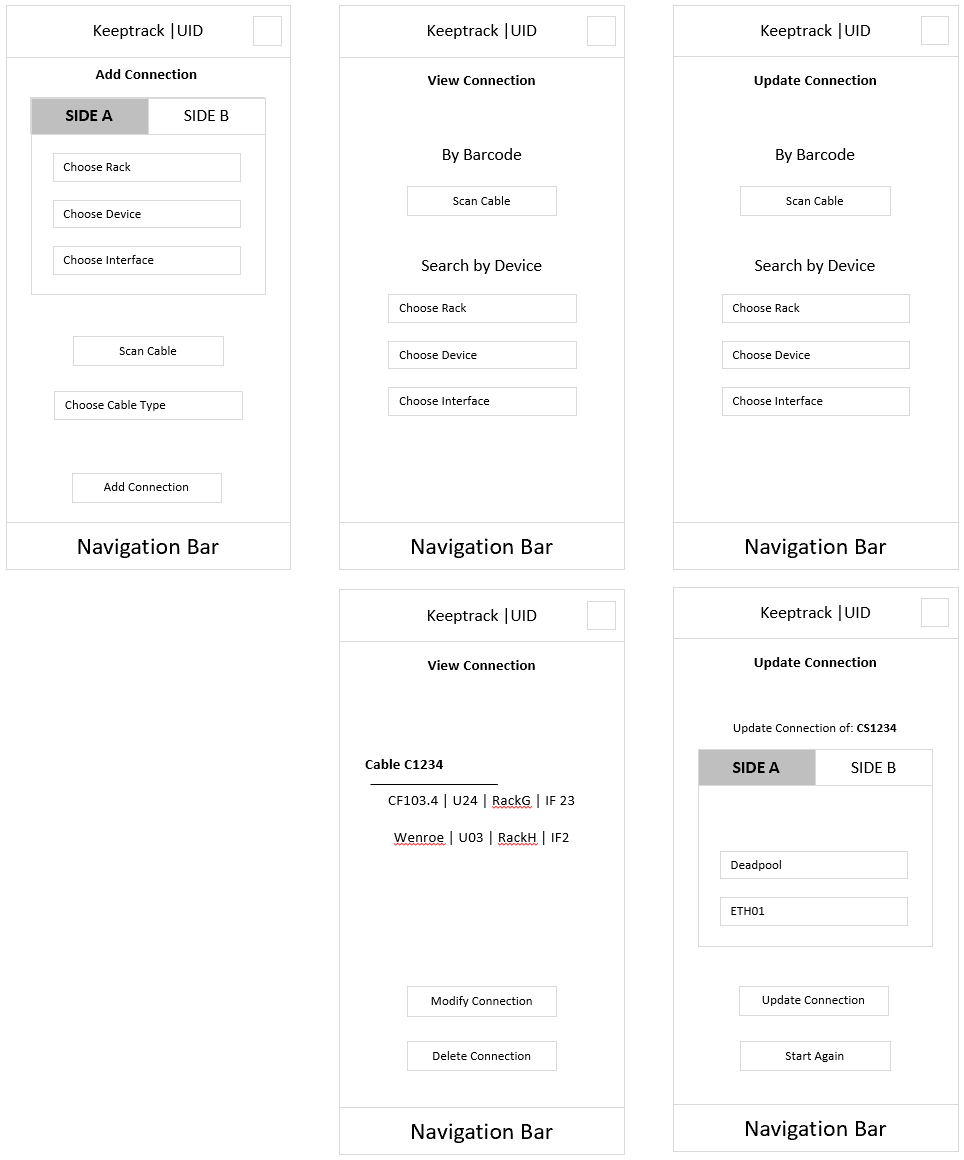
\includegraphics[width=0.75\textwidth]{images/initial_prototype_connections.png}
    \caption{Connections Screens}
    \label{fig:low_fidelity_prototypes_connections}
\end{figure}

For adding a connection between two devices (Top Left Fig.\ref{fig:low_fidelity_prototypes_connections}) the user would be presented with a tab that would allow them to select the two devices that they wanted to connect. This way it would be easy to switch between both devices whilst simultaneously not overpopulating the screen with too much data. To select a device, a user could choose a device based on a hierarchical search of sorts, first choosing the rack, then the device, and then the interface. Next, the user would need to scan a pre-existing cable with a barcode scanner. Finally, the user would choose the cable type and then add the connection. 

To view a connection, the user would have two primary methods - Either by searching by the barcode on the cable, or by searching by one of the two devices that the cable is connected to. This would then show the user the connection (Bottom Middle Fig.\ref{fig:low_fidelity_prototypes_connections}) and the devices that are connected to it, their location and interface. Finally updating a connection (Top and Bottom Right Fig.\ref{fig:low_fidelity_prototypes_connections}) would share the same initial search layout, but allow the user to change the cable device and interface terminations. This would also use the tab-based layout. 

\pagebreak

For interface management, the screens were:
\begin{figure}[H]
    \centering
    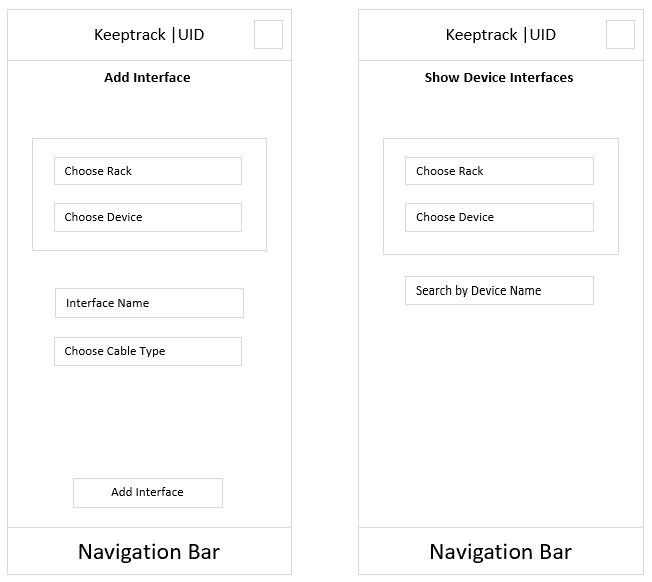
\includegraphics[width=0.50\textwidth]{images/initial_prototype_interfaces.png}
    \caption{Interfaces Screens}
    \label{fig:low_fidelity_prototypes_interfaces}
\end{figure}

Based on the initial requirements for the app, the user would need to be able to add and view interfaces. To add an interface (Left Fig.\ref{fig:low_fidelity_prototypes_interfaces}), the user would need to select the device to which they wanted to add the interface to. This would be done by selecting the rack, and then the device. Once the device was selected, the user would then be able to add the interface. This would be done by selecting the interface type and name. 

Secondly, to view a device's interfaces (Right Fig.\ref{fig:low_fidelity_prototypes_interfaces}), the user would need to be able to search for the device initially via its rack and then the device. This would then show the user the interfaces that are connected to the device. A second approach would be by searching for the device directly by its name in a text field. At this prototype stage, there wasn't a design for the interfaces themselves, but it was assumed that the user would be able to see the interface type and name. 

For device management and the side menu bar, the screens were:
\begin{figure}[H]
    \centering
    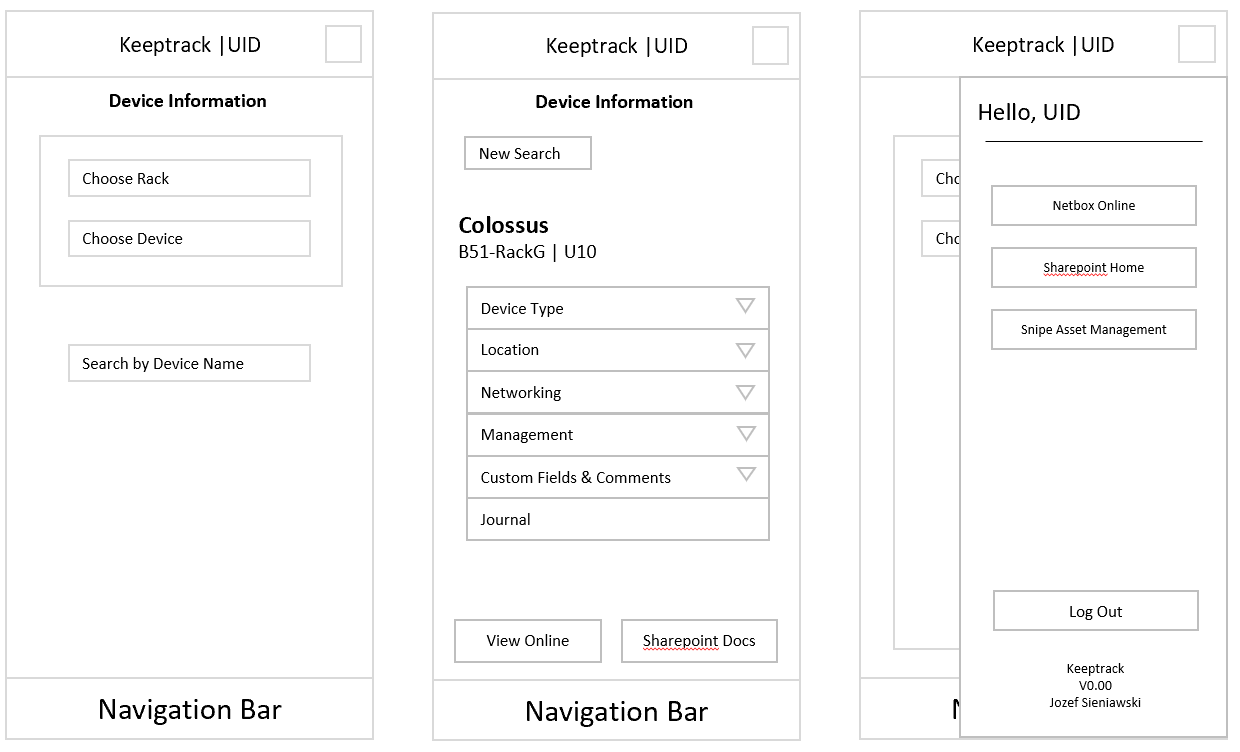
\includegraphics[width=0.70\textwidth]{images/initial_prototype_devices.png}
    \caption{Devices Screens}
    \label{fig:low_fidelity_prototypes_devices}
\end{figure}

To view a device (Left Fig.\ref{fig:low_fidelity_prototypes_devices}), the user would need to be able to search for the device by its name and again by rack then device. This would then display a new screen (Middle Fig.\ref{fig:low_fidelity_prototypes_devices}) that would show the user the device information in an expandable list. This was designed to improve upon the overwhelming amount of information that is shown on the Netbox equivalent screen. This collapsible list would allow the user to only see the information that they want to see.

The side menu bar (Right Fig.\ref{fig:low_fidelity_prototypes_devices}) was designed to be quickly accessible from anywhere in the app. This would show the current user logged in as well as navigate to other systems, e.g. online Netbox instance. Additionally, this would be where the user could log out of the app if needed.

Finally, the app itself is designed upon a multi-page layout with navigation between pages being done via a bottom navigation bar. This was chosen as it is a common design pattern in mobile apps and is easy to use. 


\subsubsection{Current State \& Interview Analysis}
\label{sec:ui_design_interview_analysis}
Following the completion of these designs, they were then shown to the interviewees as a part of the current state analysis. This was done to ensure that the base requirements were considered but also any comments on the designs themselves as well as any additional requirements that were not considered. 

As mentioned in the methodology section \ref{sec:current_state_analysis}, the interviews were conducted in person with a set of questions that were designed to elicit the current state of the school's server room. Then, the interviewees were shown related products and asked to interact and comment on them. Finally, the interviewees were shown the low-fidelity prototypes and with the context of their previous answers and opinions on related products, were asked to comment on the designs. Additionally, the interviewees were asked if there were any additional requirements that they felt were not considered.

Three interviews were conducted, each interviewee being a full-time system administrator for the School of computer science and a member of the RST team. The interviews were conducted in person, recorded and lasted approximately 45 minutes. These recordings then have been transcribed and analysed. These transcripts were then analysed using a thematic analysis approach \cite{thematicAnal}. First by reading through the transcripts, and then identifying any themes that were present. Each interviewee is referred to as Interviewees 1, 2 and 3. 

The primary themes that were identified from the interviews were:

\begin{itemize}[topsep=0pt]
    \item \textbf{Legacy systems}: Many systems in the workplace are outdated, which leads to issues with maintenance and troubleshooting.

    \item \textbf{Documentation and organisation}: Documentation is lacking, and there is a need for well-labelled and well-thought-out cabling and documentation. Interviewees suggest using a dynamic system like Netbox to help with documentation, capturing a document outlining a system's specifications, owner, and status, and implementing a journaling/auditing feature to make troubleshooting easier in the future. 
    
    \pagebreak
    
    There is also a need for an inventory system to track physical devices and use unique identifiers for each connection, as well as implementing QR codes on servers to make identifying them easier.

    \item \textbf{Adaptability and flexibility}: There needs to be more flexibility and adaptability in the team, as new people will come and go, and the system may need to be modified or expanded.

    \item \textbf{Reorganizing and re-platforming}: There is a lot of work to do in terms of reorganising and re-platforming systems. The team needs to balance outdated and modern technology and address single-point failures in the team.

    \item \textbf{Visual representation}: Interviewees suggested an AR feature for visualizing the inventory system would be beneficial. A visual representation, such as AR, is easier to relate to than data. But, it may be overly complicated to implement.

    \item \textbf{Monitoring and Maintenance}: Monitoring and maintenance are important in server management. Temperature monitoring in server rooms is essential, and the current solution isn't viable. End-of-life and warranty information should be easily accessible, and a view on Netbox of this information could be useful.

    \item \textbf{Resistance to change}: There is resistance to the idea of integrating the data centre into a larger facility, and staff members have expressed resistance to this idea.

\end{itemize}

With these themes in mind, the low-fidelity prototypes were then modified to address them and to ensure that the base requirements were considered. These modifications are outlined in the next section (\ref{sec:high_fidelity_prototypes}). 


Aside from the themes above, the most notable takeaway from the interviews was that there is a lack of documentation, with interviewee one explaining ``There's a lot of undocumented scripts, a lot of undocumented servers. There's a lot of undocumented all over." This is a core aspect that the project has aimed to address, intending to create a system that makes it easier to document and maintain the server room. 

Additionally, several design ideas were suggested by the interviewees, such as the use of augmented reality, similar to that of Cloud3DView \cite{cloud3dview}, to help visualize the server room. This was not included in the low fidelity prototypes as it was not considered a core requirement, but it was something considered as a stretch goal post the MVP. Though interviewee one described the idea as a ``very stretch goal" and ``complicated".

One core design suggestion was to implement a hierarchical search feature, similar to that of Pathfinder \cite{PathfinderMobile}, to help users find devices easier. Interviewee 1 described Pathfinders search function as `useful" and more ``interactive". Interviewee 2 also mentioned that Pathfinder's hierarchical functionality would also be great ``support wise" and that ``knowing all that information beforehand would be brilliant". Specifically, it can aid in the networking troubleshooting process, for example, DHCP configuration issues.

On a similar note, interviewee three mentioned that the low-fidelity device searching screen was too complicated and that a simple search bar would be better. Specifically, ``I'm thinking if you can find the easy way to locate the device, rather than select the Rack, the size, the room and the device from the scroll down list". 

A specific comment was made about the addition of connections, where interviewee one mentioned that being able to specify the colour of the cable would be important for troubleshooting as well as a visual aid.  

Interviewee three suggested a feature to run simple commands on devices, such as a ping command, to help with troubleshooting. This was not included in the low fidelity prototypes as it was not considered a core requirement, but it was something considered as a stretch goal post the MVP. Specifically, interviewee three mentioned, ``I would really like to check the servers status in real time and having some basic commands would be helpful".

Finally, one feature that interviewee one suggested was the addition of journaling for devices. Specifically that it would build a history of changes and fixes to issues as they arise. This was not included in the project due to limitations with the Netbox API, but something that can be considered for future iterations of the project.


\subsubsection{High Fidelity Prototypes}
\label{sec:ui_design_high_fidelity_prototypes}

Following the initial interviews, a set of high-fidelity prototypes were then created. These were created using Figma \cite{figma}, a web-based prototyping tool. Chosen due to extensive prior use and its high reputability, with the UX Design Institute describing it as the best prototyping tool \cite{figmaUX}. With Figma's prototyping features, it is possible to create interactive prototypes, these were then used to conduct further interviews, but with a more evaluative, less formal focus. These higher fidelity prototypes also include changes raised during the interview process as well as new features.

As mentioned previously, the interface has been focused on Material Design, which is described as `an adaptable system of guidelines, components, and tools that support the best practices of user interface design.'\cite{materialDesign}. It has several User Experience (UX) principles at its core (such as accessibility) that will create a user-friendly interface. Material is widely used and will give users a sense of familiarity, especially icons and GUI elements. This similarity increases learnability and reduces the user's cognitive load.

These designs were based on five core screens. Then each screen's functionality triggers a tree of other views to display data/confirmations etc. One notable difference is the removal of the interface add screen. It was decided that since it wouldn't be a task that would be done often and or in situ, it was to be removed. See the below figure \ref{fig:figma} of higher fidelity prototypes. 

These screens are:
\begin{itemize}[topsep=0pt]
    \item Add, Search and Modify Connection
    \item Device Interfaces
    \item Device Information
\end{itemize}

\begin{figure}[H]
    \centering
    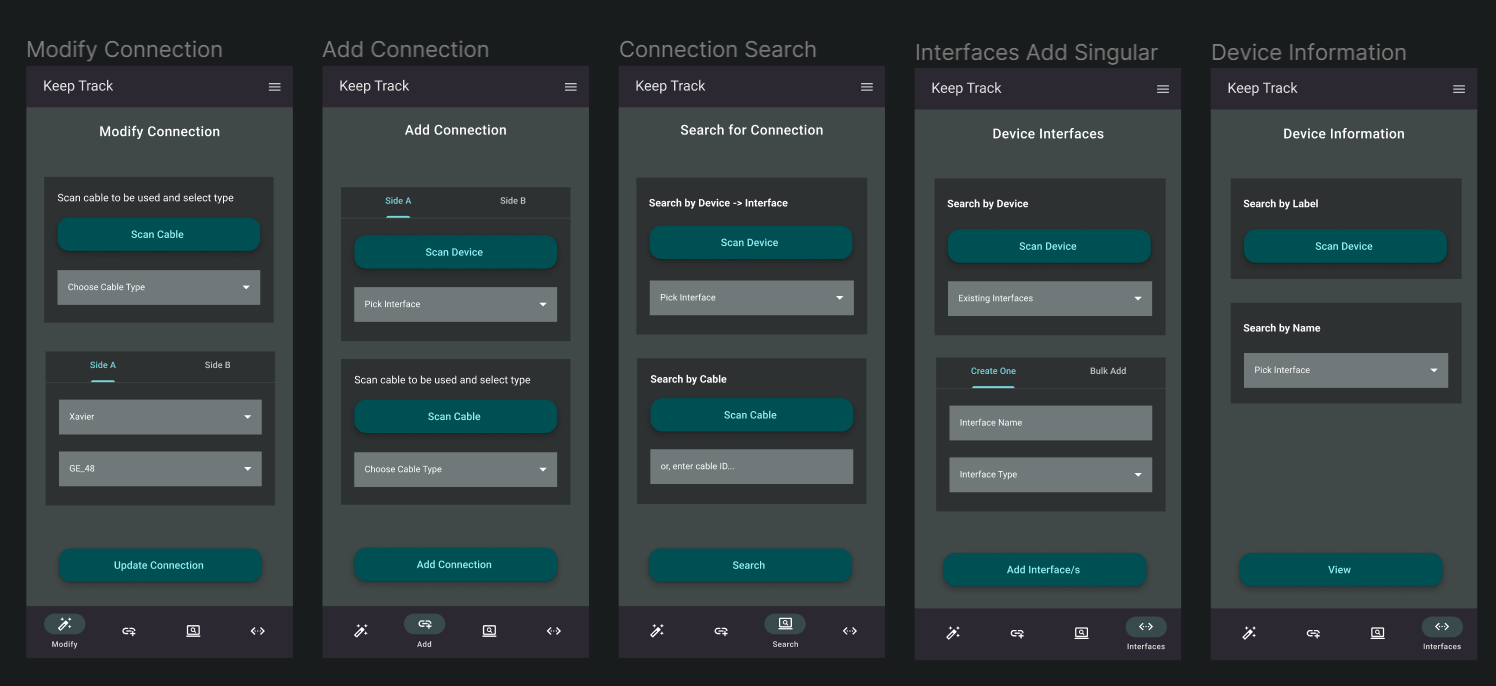
\includegraphics[width=1\textwidth]{images/figma_prototype.png}
    \caption{Figma Prototype}
    \label{fig:figma}
\end{figure}

The core features of the app remained the same but were modified to address comments made during the interviews. Primarily, the changes were focused on search methods, names and layouts of the screens. Starting with the Connection features, `Update Connection' was changed to `Modify Connection' for clarity (left fig.\ref{fig:figma} ). Further, the `Modify' flow was changed into two sections. First scanning the cable, which would then automatically fill in the cable information. Then the user has the option to modify the cable type and then in a separate section of the screen, change the devices and interfaces. A big change was the addition of the tab bar, which allows the user to switch between the two termination devices. 

This multi-section, multi-function layout was focused on the reusability of components which can complete entire operations. For example, `Add Connection' and `Modify Connection' share the same operation of searching for cables and selecting cable type. Therefore, the same component can be used for both functions. This method had the intention of increasing learnability and reducing cognitive load by reducing the number of different forms the user had to learn. This approach was used throughout the app where possible to achieve this.

To highlight the separation of sections, they were given a different background colour to the surface colour to increase contrast. Additionally, depending on the functionality of the component, their colour would change. For example, primary functions like `Add Connection' and `Modify Connection' use the primary colour, whereas dropdown menus and input fields use a secondary colour. Once again, this approach increases learnability and intuition by grouping functionality by colour.

Add connection (2nd from left fig.\ref{fig:figma}) remained primarily the same with the addition of this sectioned approach and theming. There was a removal of the search for `Rack' and `Device' and replaced with a `Scan Device' button. This change was inspired by the comments made by interviewees 1 and 3. Specifically, interviewee 1 mentioned that "we need a QR code on the front and back (of the servers)". This way they can be identified easier by one, people who are familiar with the space as well as those who aren't (Appendix \ref{sec:thematicAnalysisInterview1}[22]). 

Secondly, interviewee 3 proposed adding labels to devices to help with identification (Appendix \ref{sec:thematicAnalysisInterview3}[11]). With this in mind, the scan device button was added to allow users to scan the QR code on the device to automatically fill in the device information. 

One of the biggest changes that were made was the addition of a hierarchical search feature which was added to the `Connection Search' screen (center fig.\ref{fig:figma}). This was added to address the comments made during the interviews. Specifically, based on feedback from the use of Pathfinder, the hierarchical search feature was added to help users find connections easier (Appendix \ref{sec:thematicAnalysisInterview1}[33,34,36] as well as \ref{sec:thematicAnalysisInterview3}[18]). The hierarchical search method would allow the user to search for connections by first selecting the room, then the rack, the device and finally the interface. This would allow the user to narrow down the search results to a specific device. To implement this feature, I used a similar approach to what Pathfinder \cite{PathfinderMobile} uses, with a clickable list that changes based on the user's selection. See below for the initial designs.
\begin{figure}[H]
    \centering
    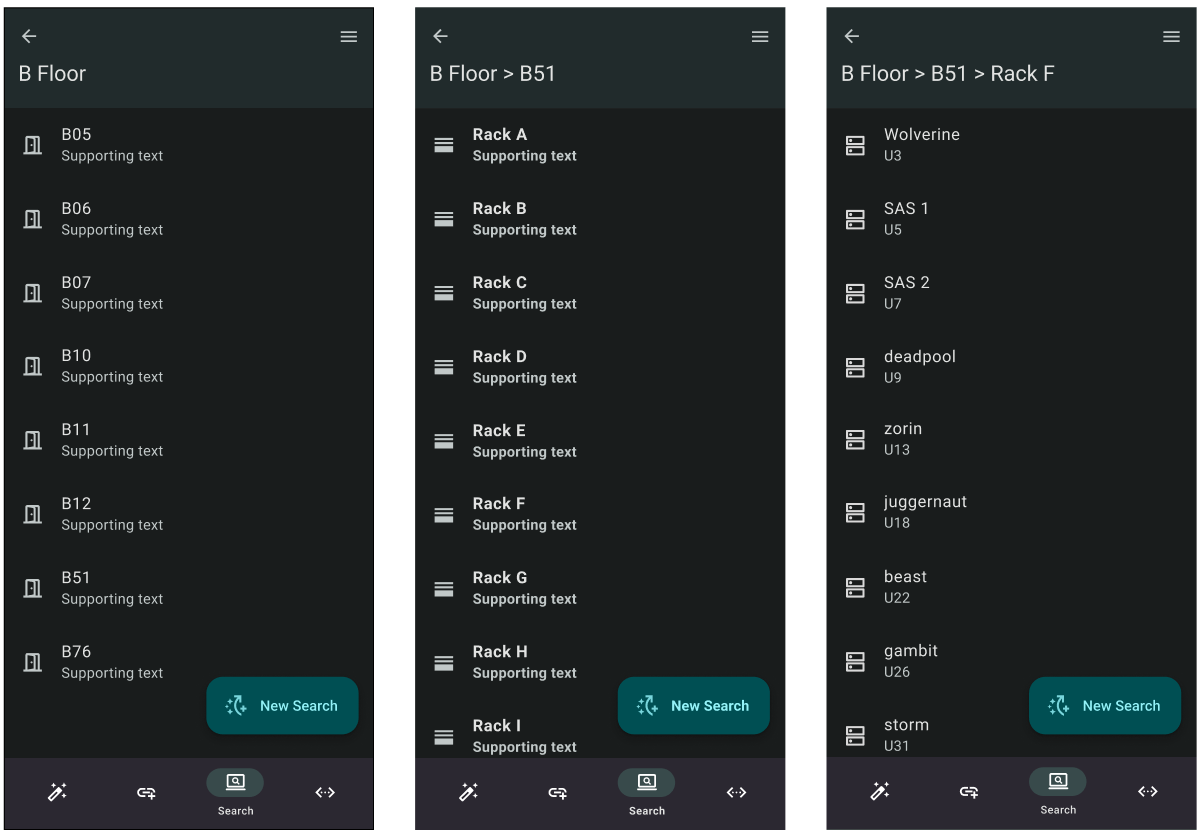
\includegraphics[width=0.75\textwidth]{images/heirarchy_search.png}
    \caption{Hierarchical Search}
    \label{fig:hierarchical_search}
\end{figure}
\begin{wrapfigure}[13]{r}{0.32\textwidth}
    \centering
    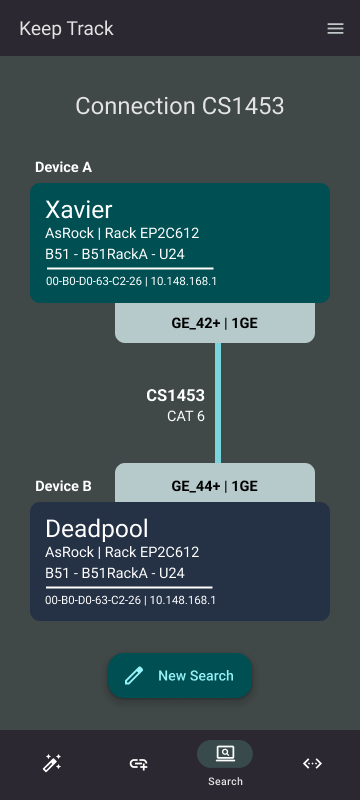
\includegraphics[width=0.22\textwidth]{images/connection_display.png}
    \caption{Connection View}
    \label{fig:connection_card}
\end{wrapfigure}
Once the user then finds the interface they are looking for, they can then select it to view the connection information. This information would include the cable type, the other device and interface, and the cable length. This information would be displayed in a card as shown in fig.\ref{fig:connection_card}. This is a core feature of the app and was designed to be as intuitive as possible. The design has taken inspiration from the Pathfinder app, which uses a similar card layout to display connection information.

One feature that was modified post-interviews was `Add Interface'. Primarily adding the capability to add multiple interfaces at once. This was inspired by the comments made by interviewee 3 (Appendix \ref{sec:thematicAnalysisInterview3}[15). 

\pagebreak
This would allow the user to create a range of interfaces at once, such as 1-48 for a 48-port switch. This would reduce the number of clicks and time taken to add interfaces. To do this, the user would select the number of interfaces they want to add, select the interface type and then define the prefix, e.g. GE for Gigabit Ethernet. The app would then create the interfaces with the prefix and number appended to the end. For example, GE1, GE2, GE3 etc. The user can toggle easily between adding one interface at a time or multiple interfaces at once by using the tab bar. This screen is shown in fig.\ref{fig:interface_add}.

\begin{wrapfigure}[20]{l}{0.30\textwidth}
    \centering
    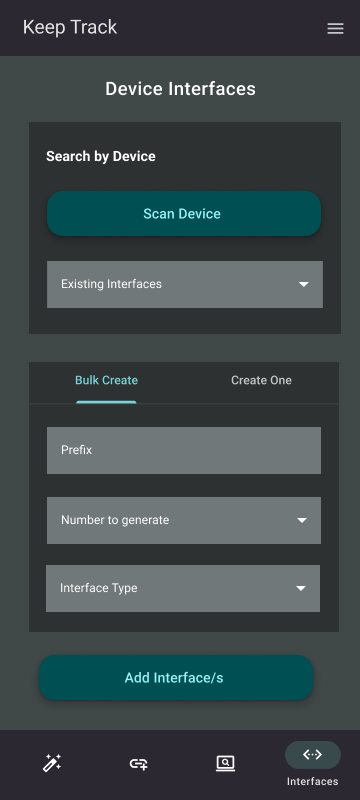
\includegraphics[width=0.24\textwidth]{images/interface_add.png}
    \caption{Add Interface}
    \label{fig:interface_add}
\end{wrapfigure}

The final screens created for the high-fidelity prototype were the `Device Information' search page and then the page to view the results. The search page (Appendix \ref{fig:device_search}) was designed to allow the user to search for devices by name but also by their QR code. This was inspired by the comments made by interviewee 1 (Appendix \ref{sec:thematicAnalysisInterview1}[22]). This would allow the user to search for devices by scanning the QR code on the device. Additionally, the second search method was added to address comments by interviewee 3 (Appendix \ref{sec:thematicAnalysisInterview3}[11]). 

As it was suggested by interviewee 2, having access to knowledge of the device would be useful when troubleshooting (Appendix \ref{sec:thematicAnalysisInterview2}[15]). This would allow the user to view the device information, such as the manufacturer, model, serial number, and other key information. Additionally, this page can also be used to show the journaling and change history as suggested by Interviewee 1 (Appendix \ref{sec:thematicAnalysisInterview1}[17,18,20,21]). This page is shown in right fig.\ref{fig:device_search}. One key decision here is the use of a collapsible list to display the information. Whilst this was already used in the low-fidelity prototype, its importance was highlighted during the interviews. The amount of information one device can have can be quite large, so having the ability to collapse the list would allow the user to focus on the information they need (Appendix \ref{sec:thematicAnalysisInterview2}[8]). 

\begin{figure}[H]
    \centering
    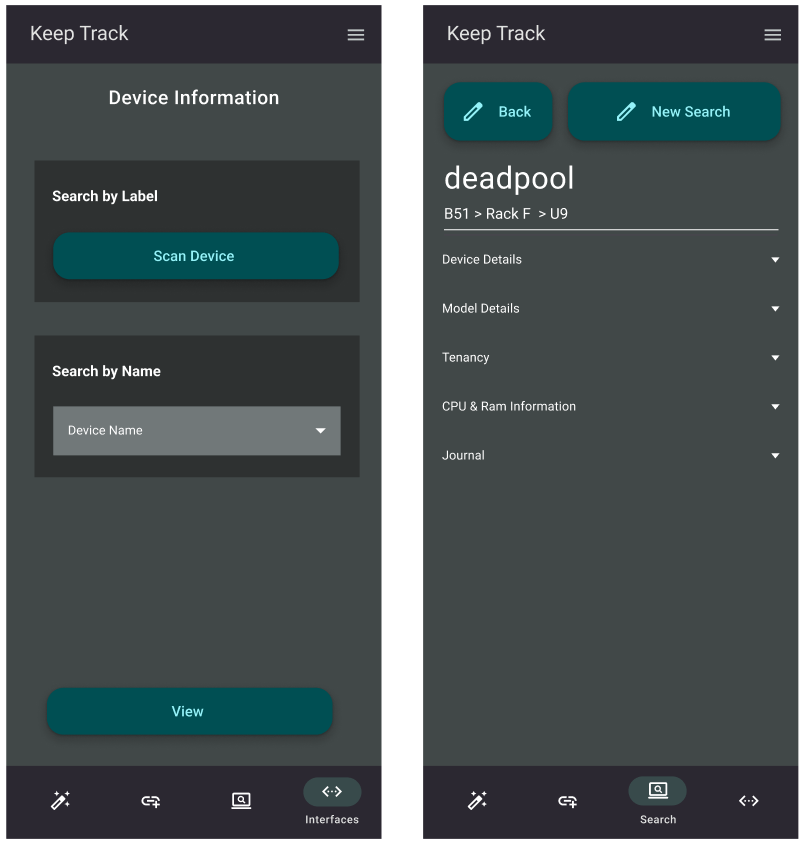
\includegraphics[width=0.5\textwidth]{images/device_info.png}
    \caption{Device Search}
    \label{fig:device_search}
\end{figure}

\subsection{Development and System Architecture}
\label{sec:development} 
Before the app could be implemented with these designs, its architecture first needed to be established. As mentioned in the methodology section (Section \ref{sec:methodology}), the app was built using Flutter. This was chosen as it is a cross-platform framework, allowing for the app to be built for both Android and iOS. The following diagram describes how the app interacts with the Netbox Instance using its REST API. These calls are processed through NGINX which is working as a reverse proxy.

\begin{figure}[H]
    \centering
    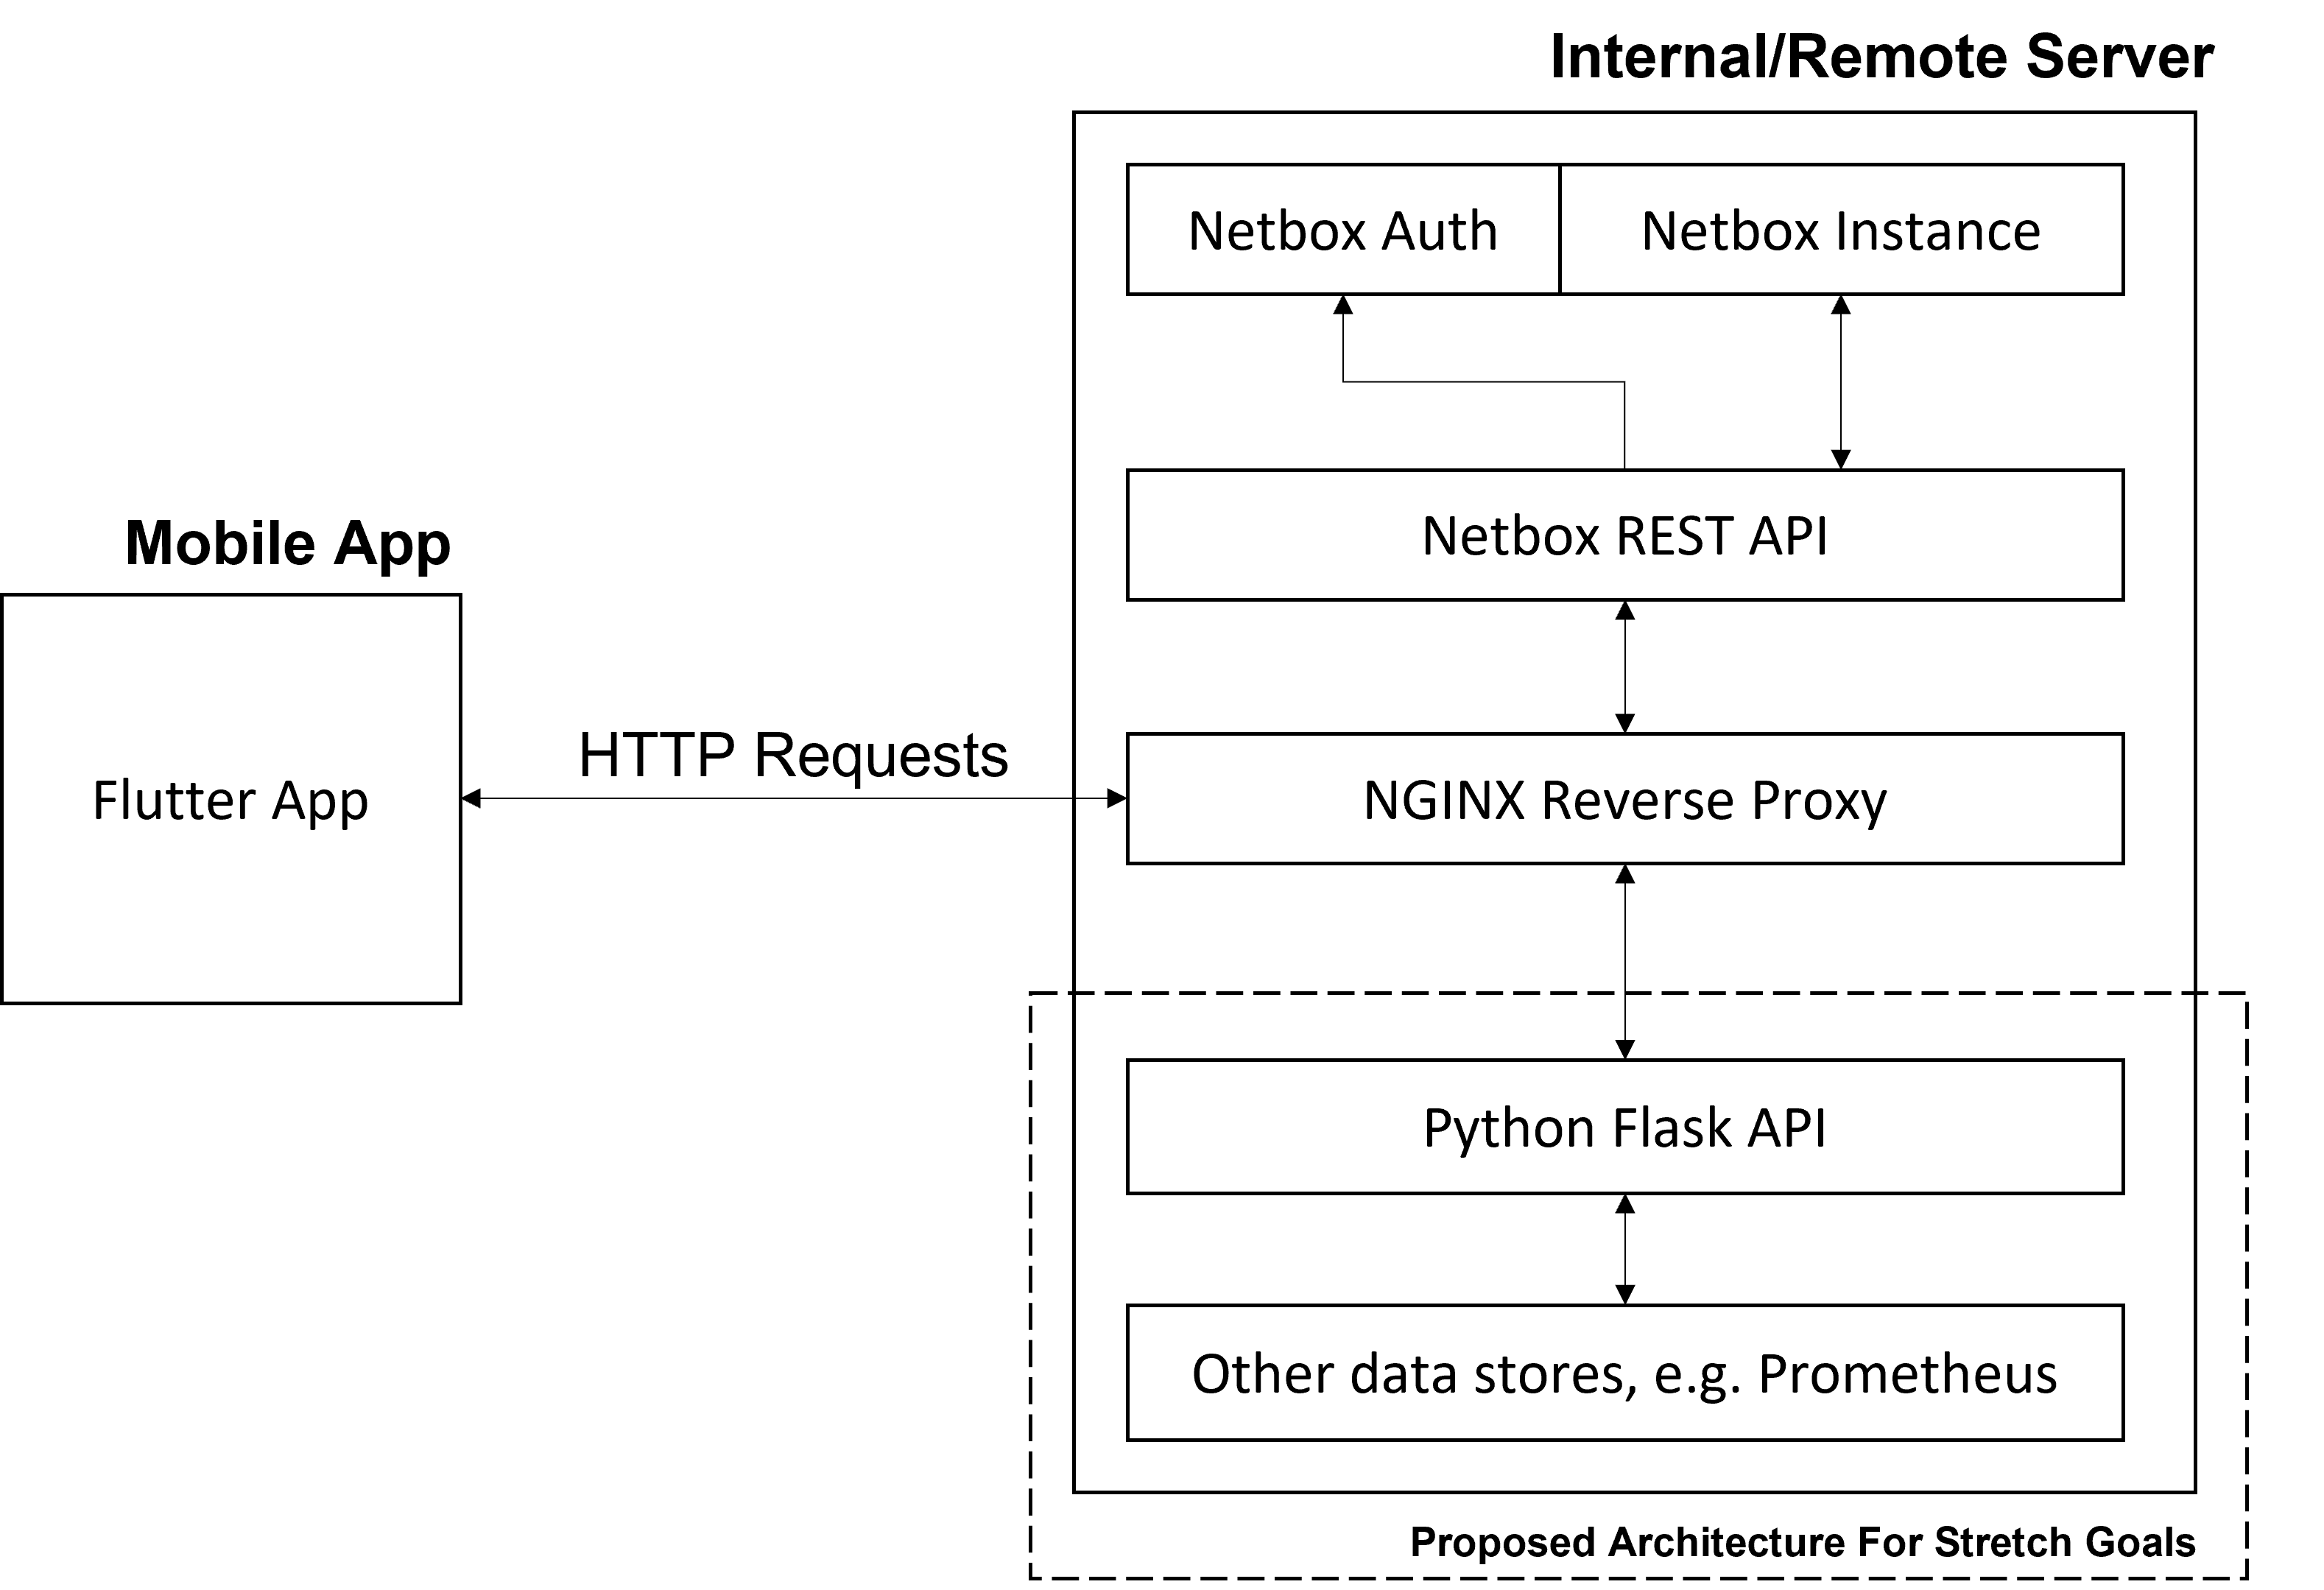
\includegraphics[width=0.6\textwidth]{images/top-level-archi.png}
    \caption{System Architecture}
    \label{fig:architecture}
\end{figure}

The app uses Netbox's inbuilt Django user authentication system, which allows for tokens to be created via an API call. This token is then used to authenticate the user to fetch data and make changes to the Netbox instance, returning any errors should a permission problem arise. For proposed stretch goals, should the app feature more information or processing, the requests will still go through the same NGINX reverse proxy but to a different proposed API endpoint. In this case, the API would be built using Python and Flask \cite{flask}. 

The app has been structured using a Data Access Object (DAO) pattern\cite{dao}, to separate the data access from the logic. In a way, replicating the data objects that Netbox uses itself. This allows for the app to be easily extended and modified in the future. This is especially important with the possible addition of features and modifications to the Netbox API.

Further, there is a separation between views, API calls and providers. This gives a more modular structure and provides more maintainable code, especially as requirements change, or Netbox updates/changes. Additionally, in the spirit of Open Source Software, the code is stored on GitHub \cite{keeptrackgithub} and has utilised environment variables to store sensitive information so that other developers can easily implement their instance of the app.

\section{Implementation}
\label{sec:implementation}
As mentioned in the methodology section (Section \ref{sec:methodology}), the app was built using Flutter and its Dart programming language. Flutter enables the app to be built for both Android and iOS whilst also having a single codebase. By using Flutter's built-in libraries as well as third-party libraries, the requirements of the app were met. The following is a list of third-party libraries used in the app:
\begin{itemize}
    \item \textbf{flutter\_dotenv} - Used to load environment variables from a .env file. This is used to store sensitive information such as the Netbox API URL and the API token \cite{dot_env}.
    \item \textbf{flutter\_secure\_storage} - Used to store the API token securely on the device. This is used to authenticate the user to the Netbox instance \cite{secure_sec}.
    \item \textbf{flutter\_launcher\_icons} - Used to generate the app icon for both Android and iOS \cite{icon_launch}.
    \item \textbf{mobile\_scanner} - Used to scan QR codes and return the result \cite{barcodeScannerPlugin}.
    \item \textbf{dropdown\_search} - Used to create the dropdown search bar for searching for devices, sites, and racks \cite{dropdown}.
    \item \textbf{searchable\_listview} - Used to create the list of devices and allow for it to be searchable. This is used in the device search page \cite{searchable}. 
\end{itemize}

Additionally, based on the findings from J.Myka et al's comparative analysis of data entry method on mobile devices \cite{myka2019comparative}, the app uses a varying number of input fields based on the type of data being entered. For example, when searching for a device by its number, the app shows a numerical keyboard only. Additionally, the use of drop-down menus and filtering lists are used through the app to reduce the amount of data the user needs to scroll through.

Below are the final implementation screenshots of the app. The first screenshot (Left fig.\ref{fig:login}) is the login page, where the user can enter their Netbox credentials and log in. There is a range of functions that are run at the route of the app to ensure that the phone has an internet connection, the user is logged in and the token is valid. The user is redirected to this login page by default if the login credentials are invalid. The second screenshot (Right fig. \ref{fig:login}) is the sidebar menu, this can be accessed from any root page. This shows the user's username, and the option to use dark and light modes as well as the current Netbox domain. Finally at the bottom of the menu is the app log-out button.

\begin{figure}[H]
    \centering
    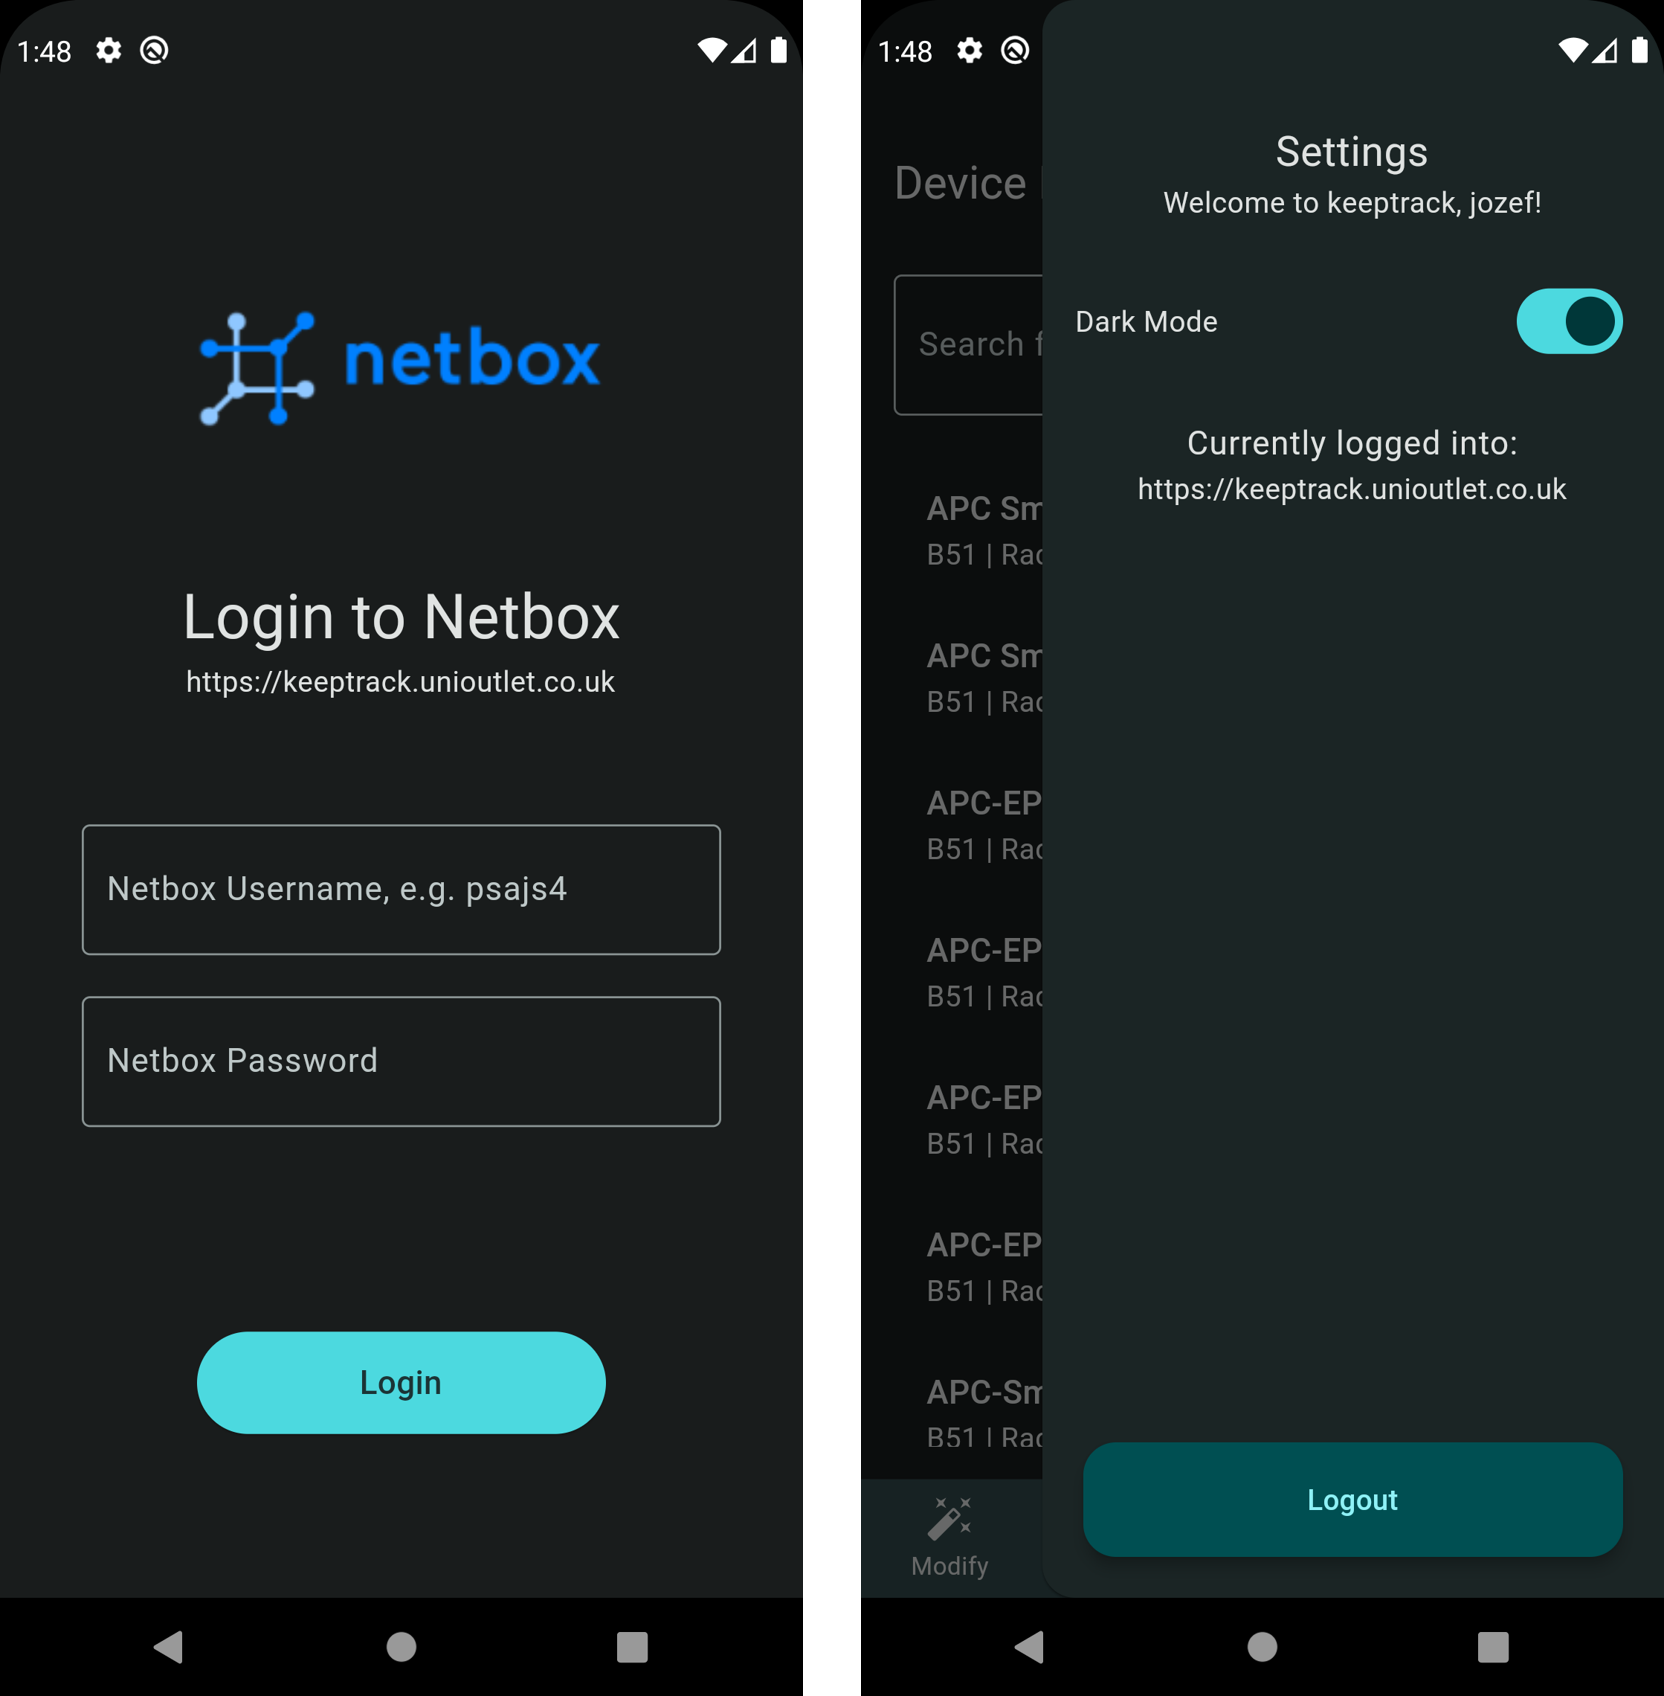
\includegraphics[width=0.46\textwidth]{images/final_login_menu.png}
    \caption{Login Page and Side Menu}
    \label{fig:login}
\end{figure}
By default, the user is shown the search connection page if/after they have logged in (Left fig.\ref{fig:search_connection}). This page allows the user to search for a device either by hierarchy or by label QR code/number. For searching by hierarchy, the user first selects the location, e.g. floor/room etc, then the rack/desk, the device and finally the interface. An example of the list is shown second from left fig.\ref{fig:search_connection}. Additionally, a screenshot showing the list of interfaces (2nd from right fig.\ref{fig:search_connection}) shows the use of a chip icon to show what devices are connected and what is not. If the user clicks on an interface that isn't connected it redirects the user to the add connection page with one side auto-populated with this interface and device. Finally, once the user has scanned/searched for the connection desired - they are shown the connection information page (Right fig.\ref{fig:search_connection}). This page shows the information on the connection, the devices and interfaces involved as well as the cable information. The user can also delete the connection and go directly to the modify connection page from this page.

\begin{figure}[H]
    \centering
    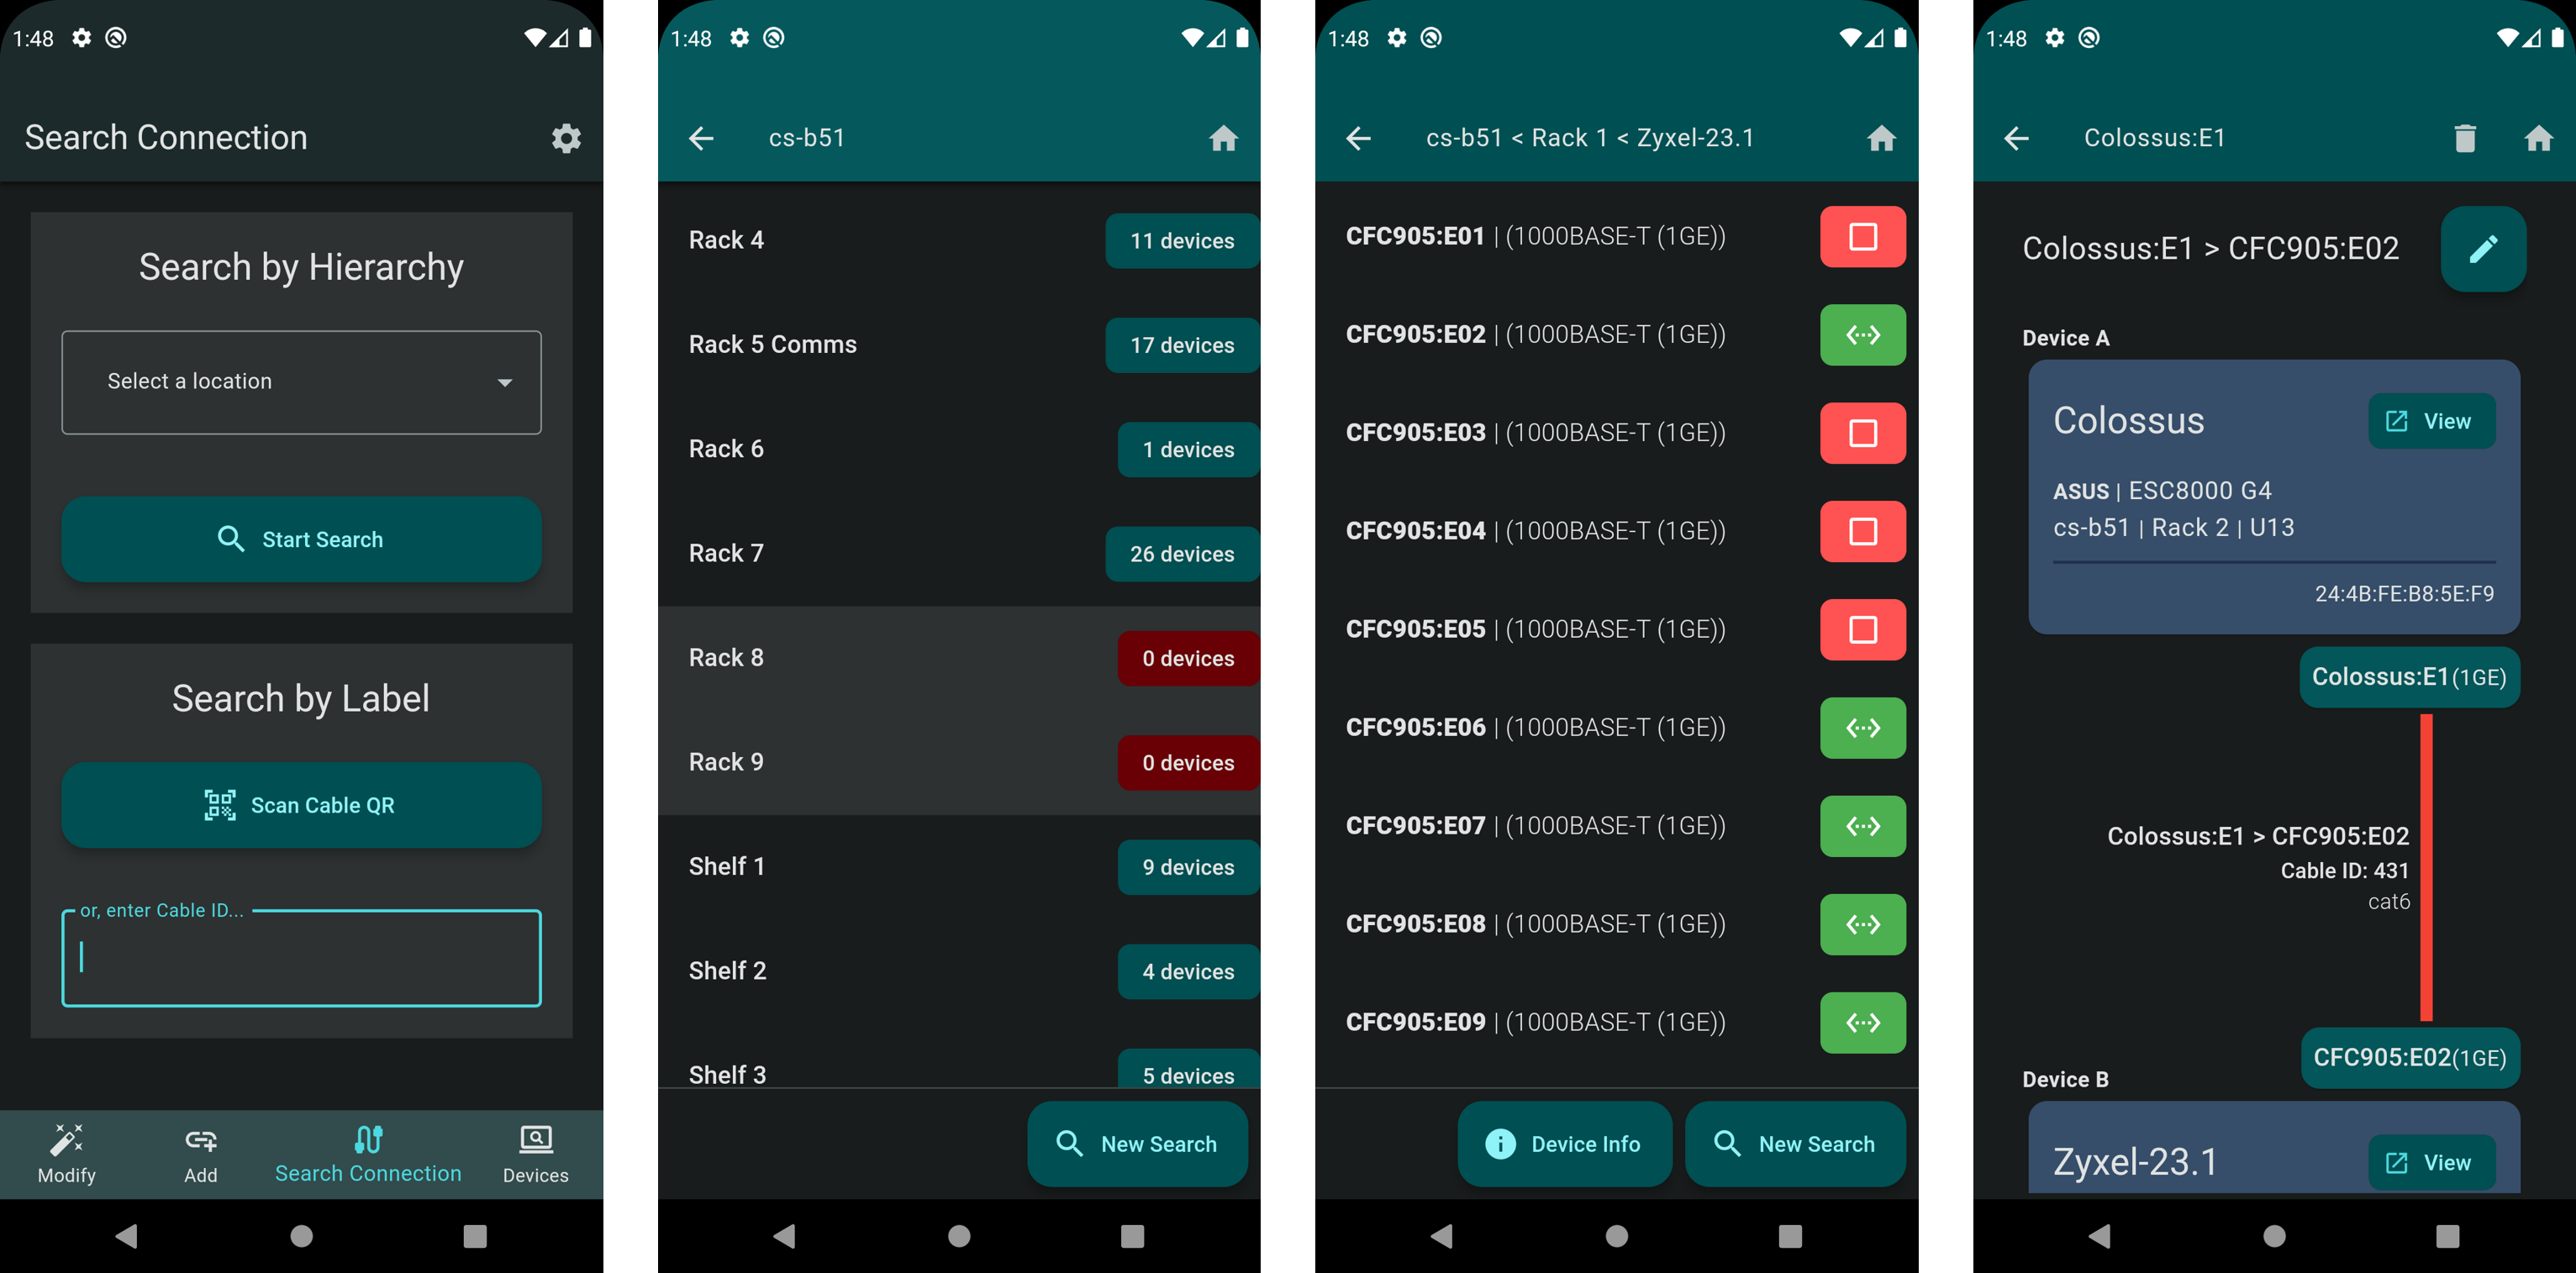
\includegraphics[width=0.9\textwidth]{images/final_search.png}
    \caption{Searching and Viewing a Connection}
    \label{fig:search_connection}
\end{figure}

The add connection page (Left fig.\ref{fig:add_connection}) remained fairly similar to that in the high-fidelity prototypes. The primary change is the focus on cable colour, which is used to identify the connections VLAN. The user chooses both devices A and B from a popup modal list search which then loads in that device's free interfaces. The user then chooses the interface for each device and the cable colour and type. The user is then shown a confirmation dialogue showing the connection description and cable ID.  

\begin{figure}[H]
    \centering
    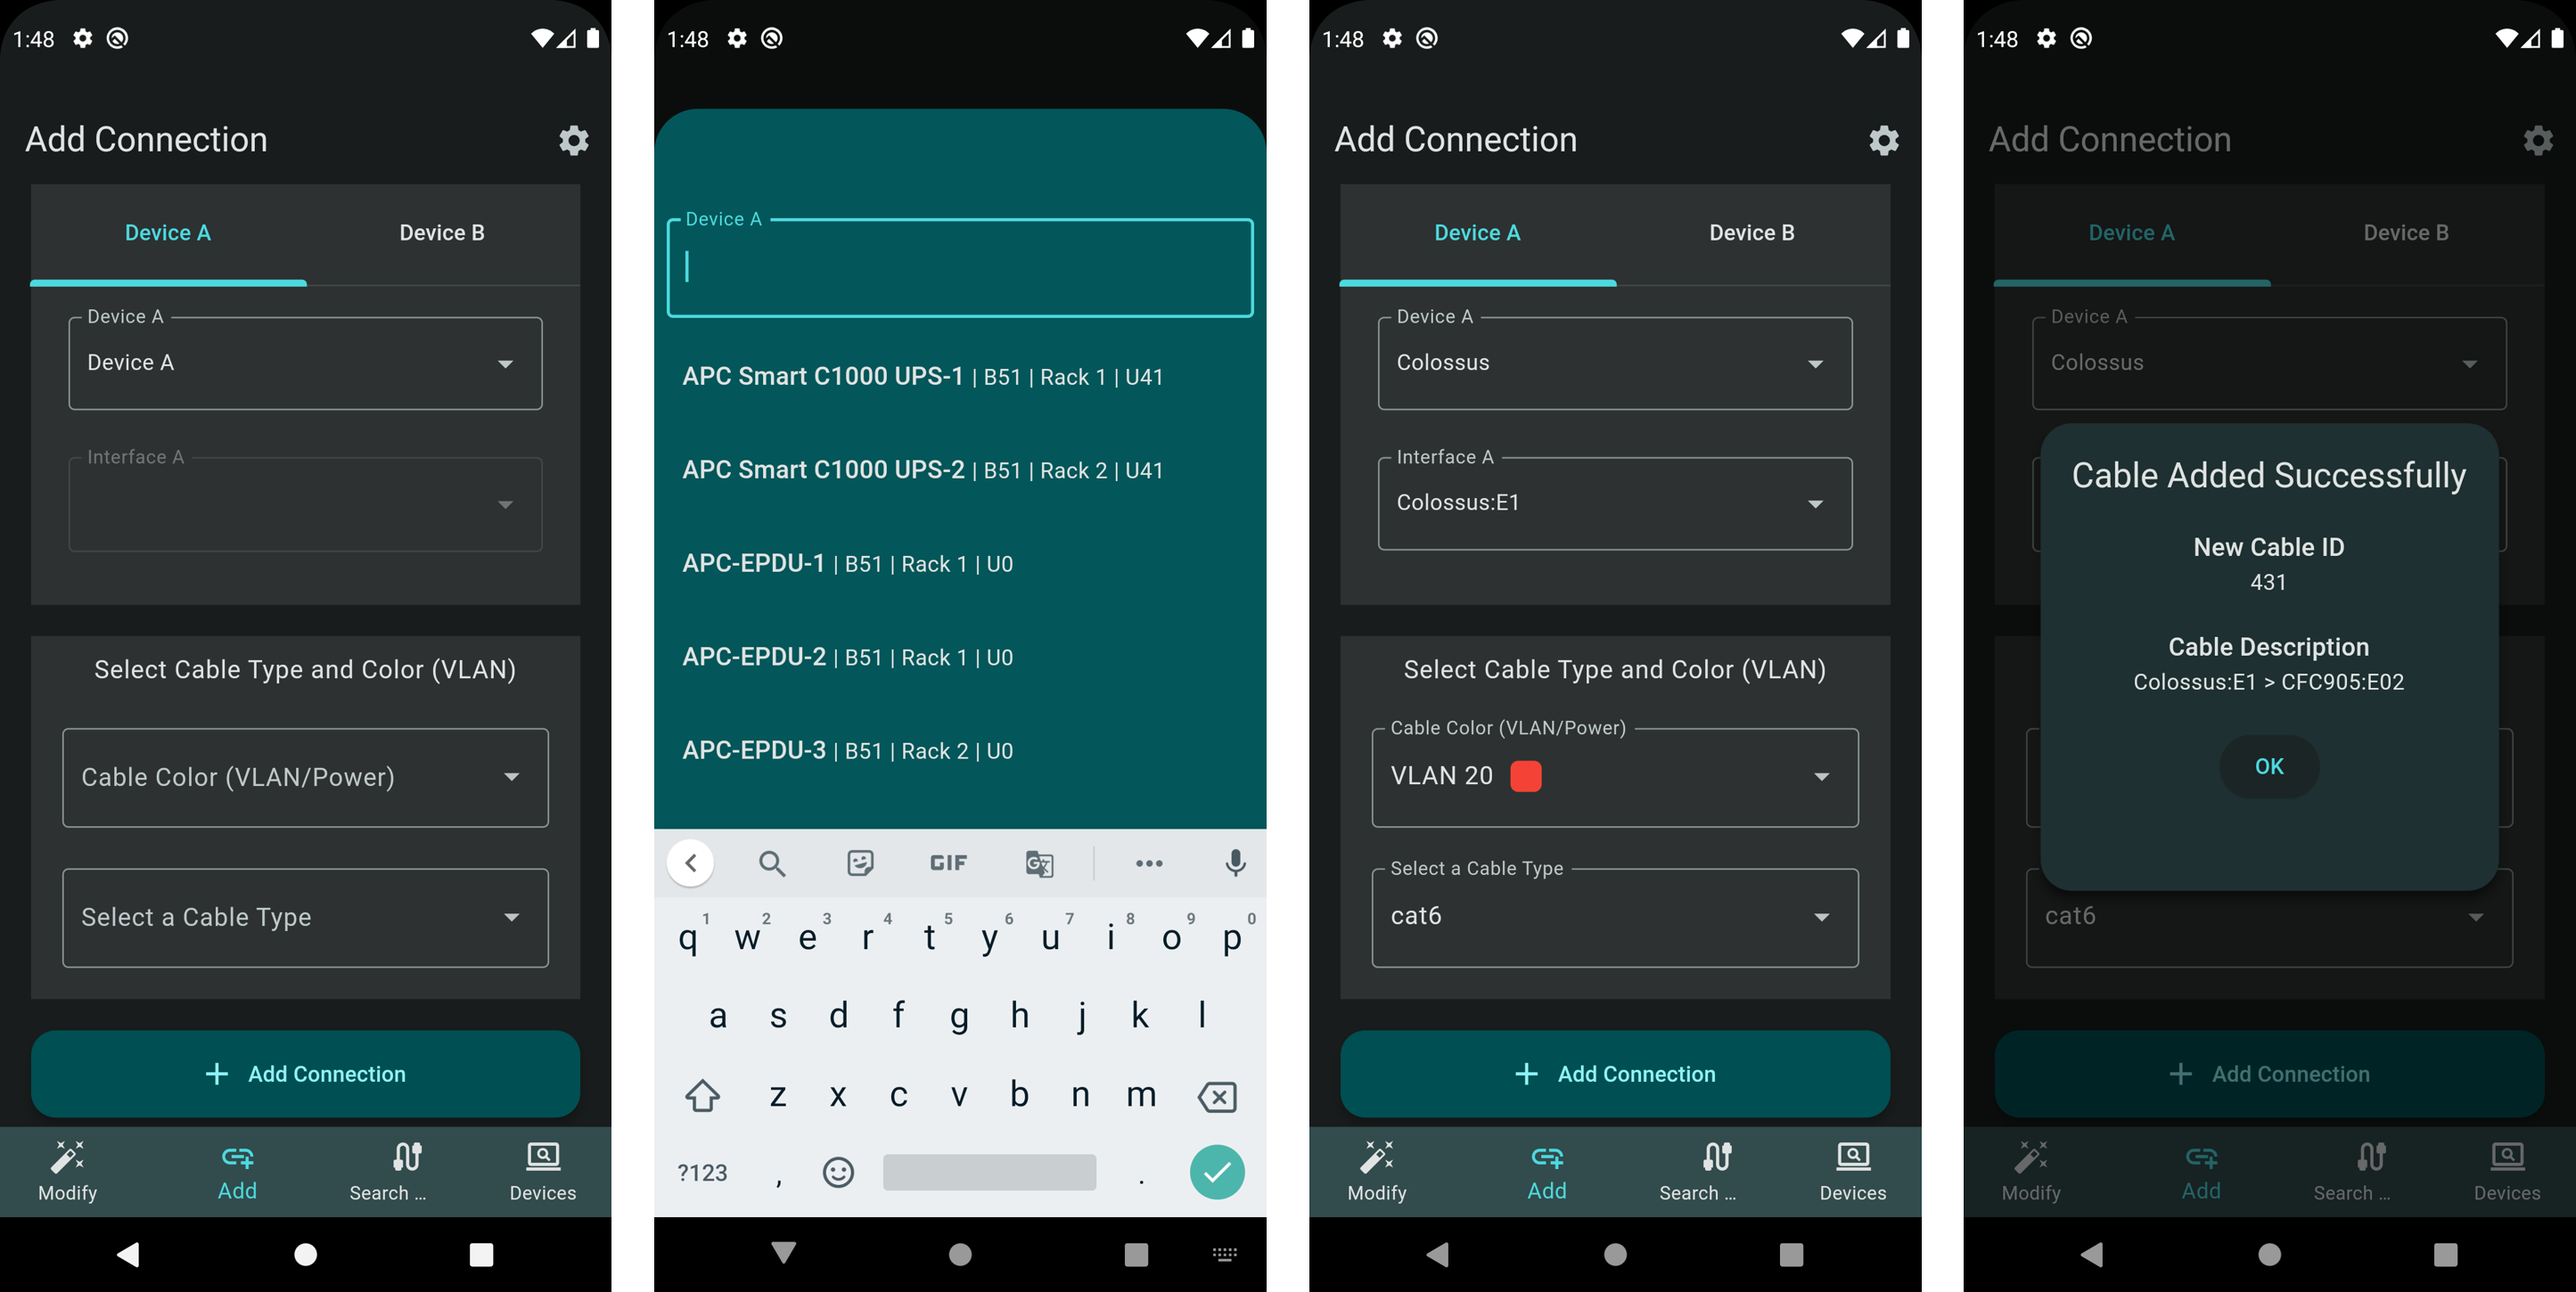
\includegraphics[width=0.9\textwidth]{images/final_add.png}
    \caption{Adding a Connection}
    \label{fig:add_connection}
\end{figure}

 
To modify a cable (Left fig.\ref{fig:modify_connection}), the user can either scan the existing cable ID or type one in - On scan/type submission, if the cable exists the UI is populated with the cable information. This includes the cable description, cable ID and cable colour. The user can then choose from a tab view of the cable termination devices and interfaces. The user can then choose the new termination device and interface and submit the changes. Here the app will automatically generate the new Cable Label with the scheme `DeviceA:InterfaceA \verb|>| DeviceB:InterfaceB'. This was to create a homogenous naming scheme and follow advice from the paper written by the CPNI \cite{cpni}. The user is then shown a confirmation dialogue showing the connection changes, and the user can then confirm the changes. Then, the API deletes the existing cable and creates a new one with the new information. Once completed the app loads the new connection automatically with the new cable ID. One big change here is that the user can now only modify the cable termination device and interface. This is due to the change in the approach to labelling cables. The cable itself is a fixed entity, so its colour and type should not be changed. This is covered more in-depth in the related technical work section (Section \ref{sec:technical}).

\begin{figure}[H]
    \centering
    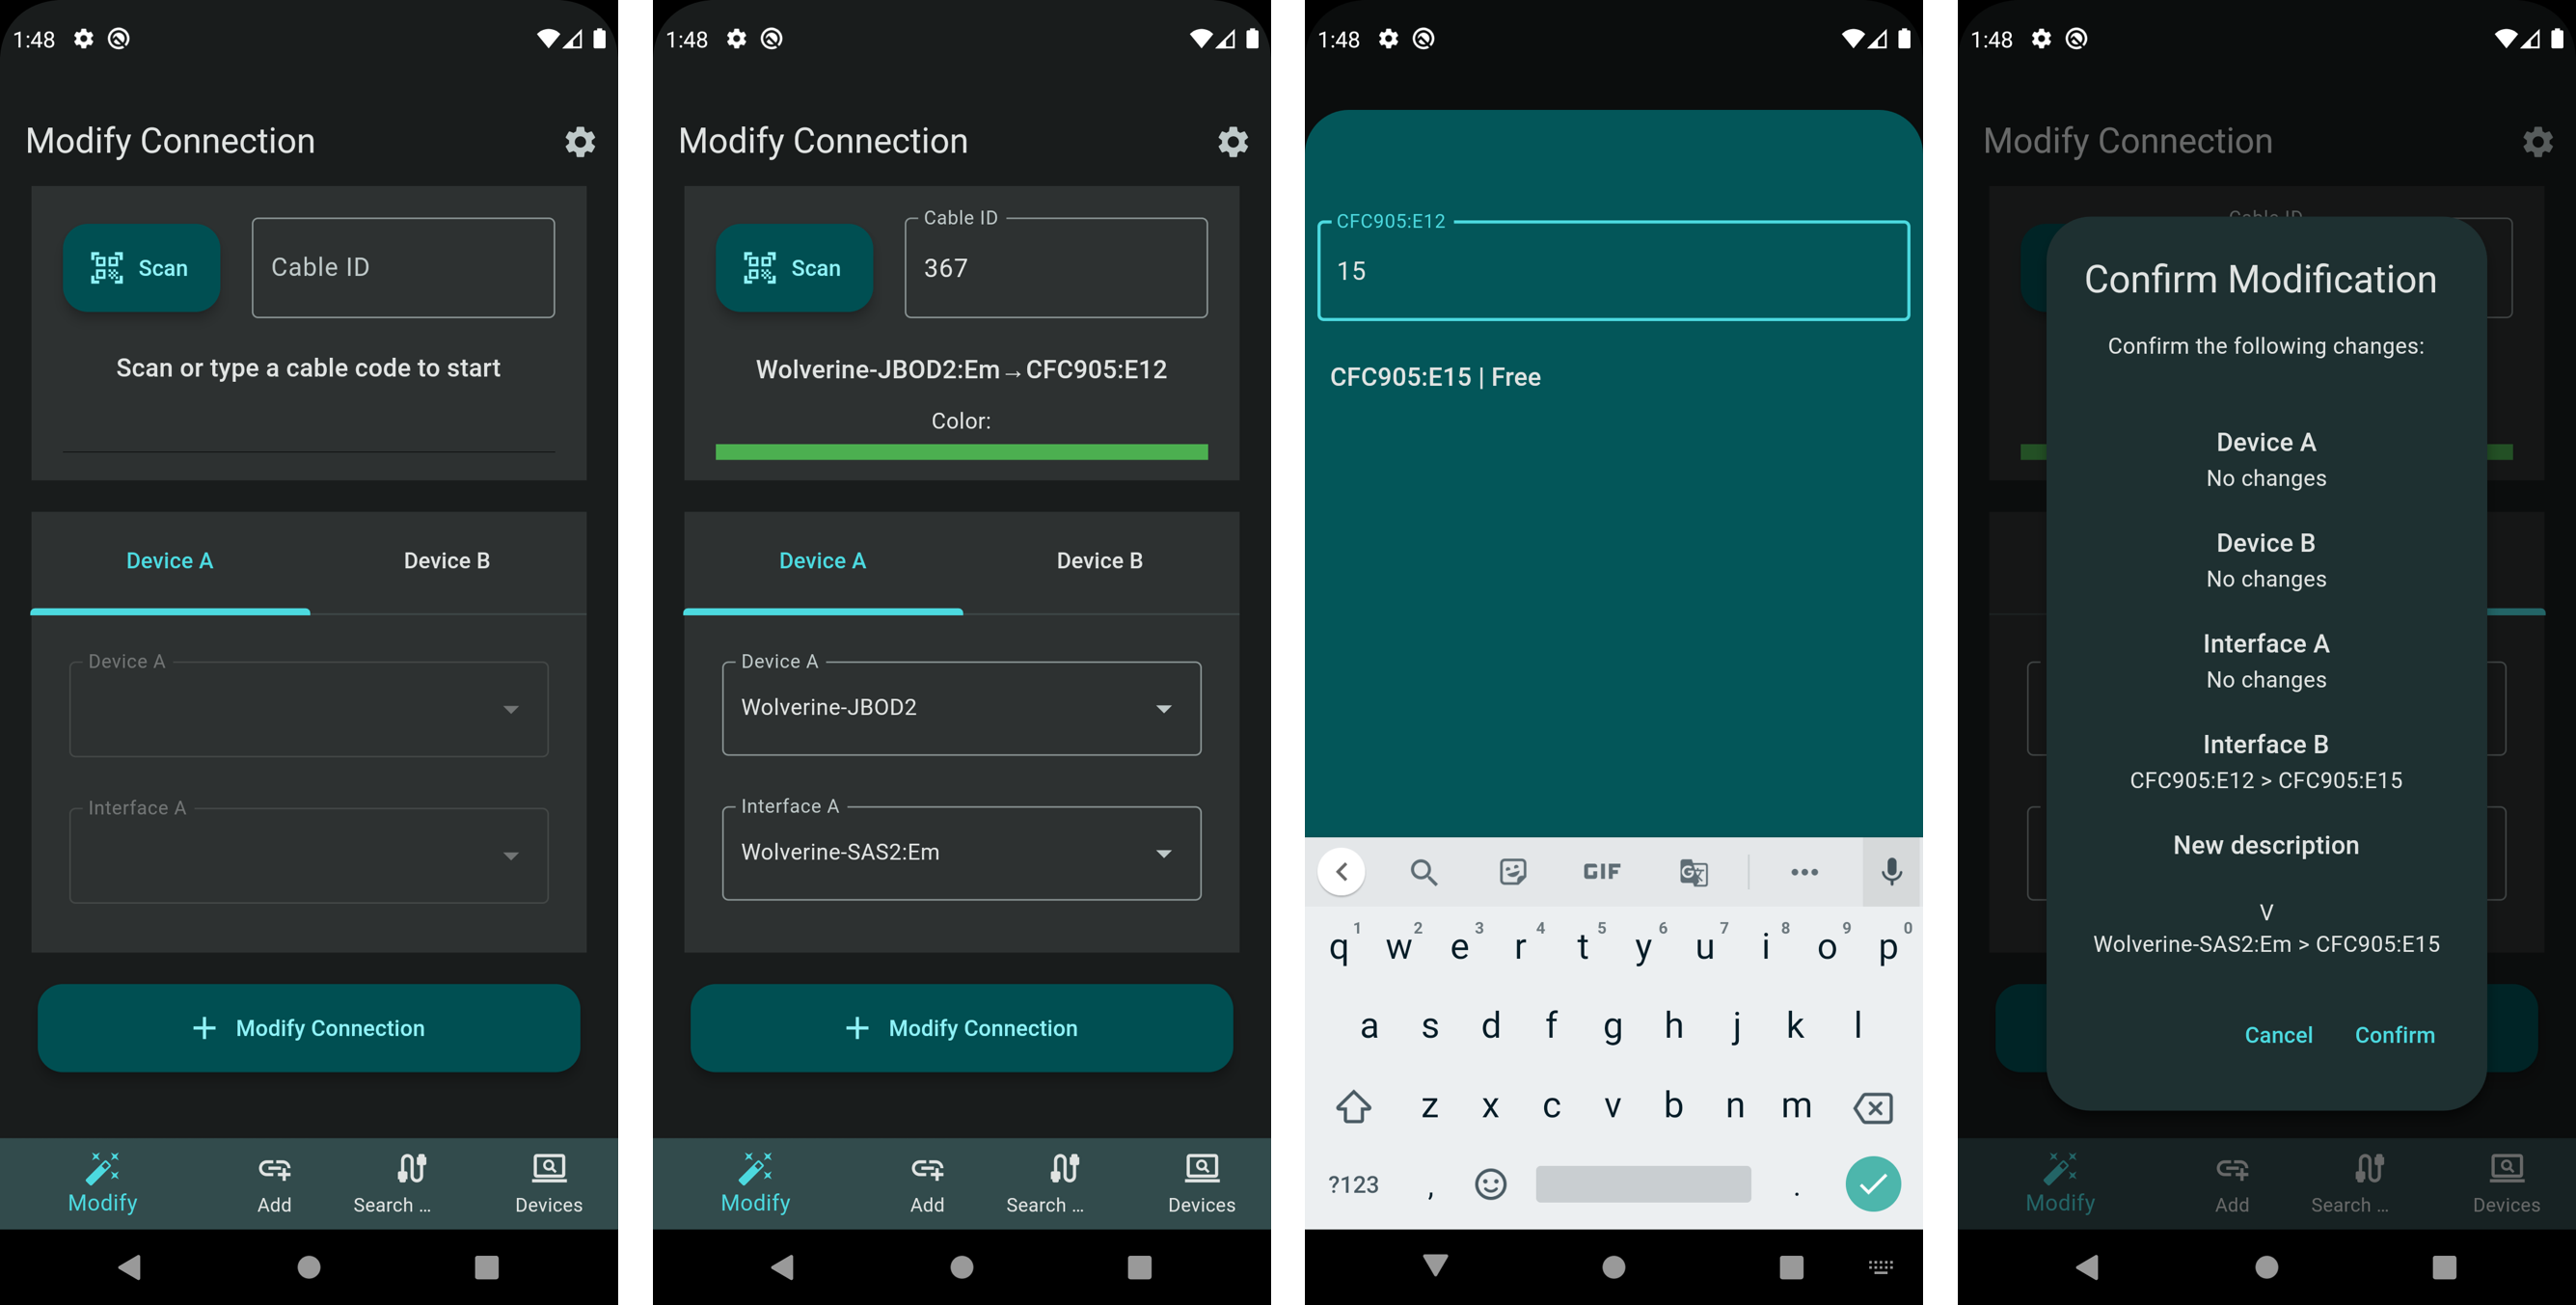
\includegraphics[width=\textwidth]{images/final_modify.png}
    \caption{Modifying a Connection}
    \label{fig:modify_connection}
\end{figure}

Finally, the device search page (Left fig.\ref{fig:device_searhc_and_view}) is the page that allows the user to search for a device by name or label, and as the user searches the list filters automatically. Then on the selection, the user can view the information associated with the device (Right fig.\ref{fig:device_searhc_and_view}), such as device details, model information, tenancy, power and CPU/RAM information. This feature partially utilises the Custom Fields feature in Netbox and so the app can be easily extended to include more information.

\begin{figure}[H]
    \centering
    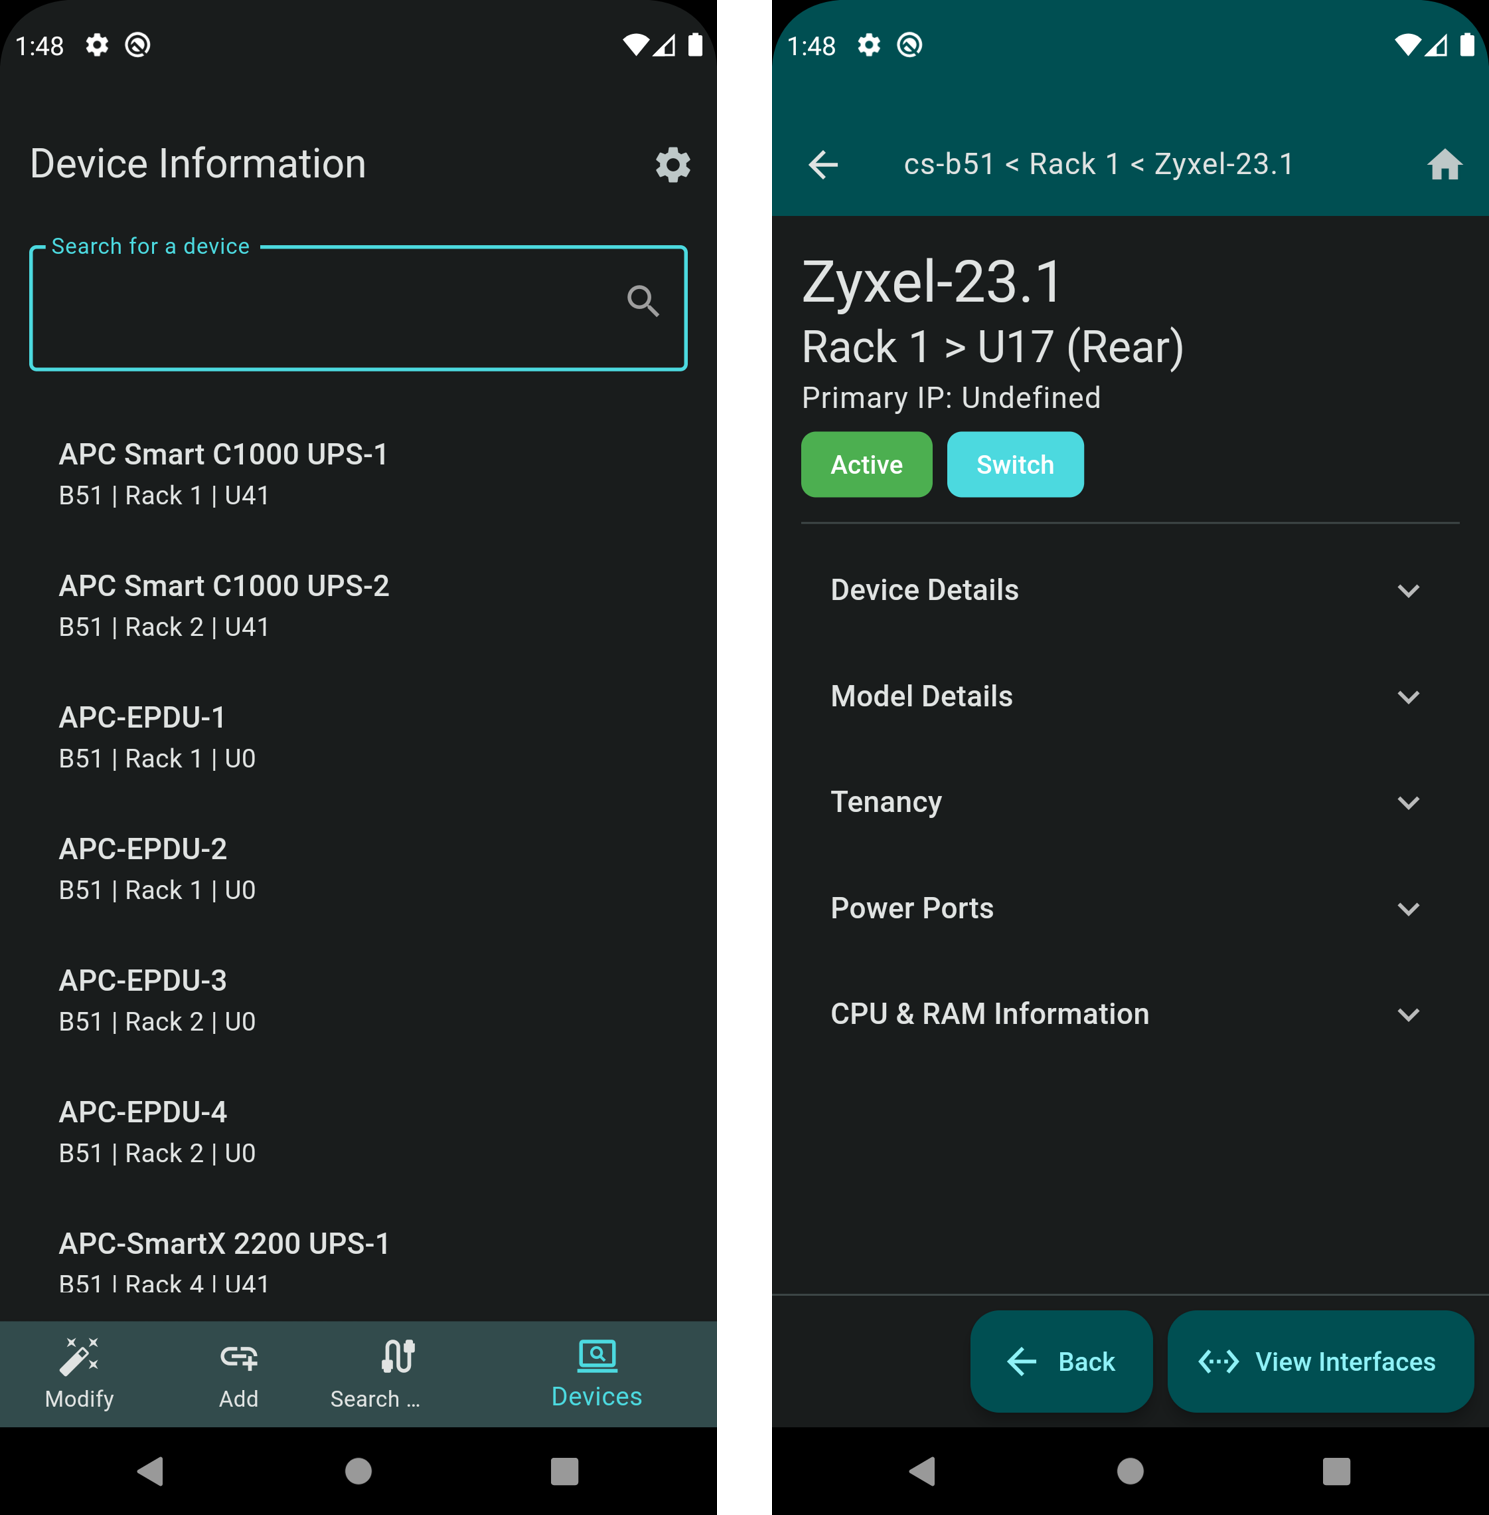
\includegraphics[width=0.5\textwidth]{images/final_device.png}
    \caption{Searching for a Device}
    \label{fig:device_searhc_and_view}
\end{figure}

\subsection{Challenges and Technical Issues}
\label{sec:challenges}

One of the primary challenges that were encountered during the development of the app was the use of `futures' and asynchronous programming. This was because the app's entire structure is based on the use of futures and the data being returned from the Netbox API. Whilst doing a few API calls it was straightforward, but due to the amount of data that is returned from the API, the structuring of the code became more complex. For example, the device search page lists over 300 devices, meaning that the data that is fetched from the API is quite large. This occurs in most places in the app and had to be made efficient as possible. The app uses two approaches, one where the UI waits for the data to be returned and then displays it, and the other where the UI is displayed first and then the data is fetched and displayed. The latter approach is used in the device search page, as it allows the user to start searching for devices as soon as the page is loaded. The previous approach is used in the add connection page, where the interfaces are fetched and displayed once the user has selected a device. 

The modify connection page (Left fig.\ref{fig:modify_connection}) took the most time to implement due to a bug that exists in the Netbox API (at the time of writing). Whilst the Cable object API endpoint allows for the modification of a cable via REST PATCH and PUT request methods, there exists a bug which causes a Django Exception. I raised a bug report on GitHub \cite{netboxBug} 2 months before the submission of this project, but it has not been resolved. Therefore, the current solution to modify a cable is to delete the cable and then create a new one. This is not ideal, but it is the only solution at the moment. 


\section{Evaluation \& Testing}
\label{sec:evaluation}
Once the app was completed, I conducted a user study with 3 participants to evaluate the implementation and design. The process of this study is outlined in the methodology section \ref{sec:user_observations_and_interviews}. Below are the observations and changes that were made to the app based on the feedback from the participants. For the entire list of findings, please see Appendix \ref{sec:appendix_observations}. 

The primary changes were focused on form entry, with all three observations having comments on the entry of data into the app. The main changes were the addition and changes to the labels, hints and error handling around the text boxes and drop-down menus. These changes were made to make the app more intuitive and easier to use and specifically address points 1, 9, 10, 14 and 15 (Appendix \ref{sec:user_observations_and_interviews}). 

Additionally, there were a few bugs that were found during the user study, which were fixed. Specifically, on the modify connection page there was a bug where a cable's terminating interfaces were not being loaded correctly to the fields (Appendix \ref{sec:user_observations_and_interviews}[8]). Secondly, on the add connection page, there was a bug where if there was an error in the entry it would show a white dialogue rather than the error itself (Appendix \ref{sec:user_observations_and_interviews}[13]). Finally, there was a bug identified on the search by connection page where the location search field was not working correctly (Appendix \ref{sec:user_observations_and_interviews}[2]). These bugs were fixed and the app was retested to ensure that they were fixed.

\pagebreak

Finally, there were a set of feature and design suggestions that were made by the participants. Some of these were implemented, specifically, points 3, 6, 7, 11, 12 and 19 (Appendix \ref{sec:user_observations_and_interviews}). Other suggestions were not implemented due to time constraints and or technical limitations, such as points 4 and 5. Primarily a good suggestion was to integrate the app with a printer system to allow for the printing of labels (Appendix \ref{sec:user_observations_and_interviews}[20]). This would make the labelling of cables much easier and quicker. However, this would require significant research and development time to implement.

Once these suggestions and changes were made, the app was retested to ensure that the changes did not break any functionality. This then made the final version of the app which is shown in the implementation section above (Section \ref{sec:implementation}).

To test the app during its development and final implementation, a full run-through of all its features was conducted. This was done to ensure that the app was working as intended and that there were no bugs. This was done by myself and confirmed via the observations and interviews conducted during the user study. To ensure that the app was working as intended, I had a live Netbox instance running on a separate machine and the app was connected to this instance of Netbox. This allowed me to test the app as if it was being used in a real environment. For example, if a connection was added, ensure it was added to the Netbox instance and with the correct information. 

Additionally, to ensure that the API calls were working correctly, I used the Postman application to test all the calls the app was making. This allowed me to see the response from the API and ensure that the app was receiving the correct data. Additionally, Postman provided great aid in the development of the app, as it allowed me to test the API calls and see the response before implementing them in the app.

Aside from the bug mentioned in section \ref{sec:challenges} and the impacts it had on the `Modify' connection feature, the app has been completed without any major issues. The app is fully functional and can be used in a real environment. 

In regards to the functional requirements specified in section \ref{sec:func_spec}, the app meets all of them, but with some slight changes. Specifically, for requirement \ref{spec_asset_5}, the app no longer needs the ability to scan barcodes. Further, requirement \ref{spec_asset_3} is not fully met as the app only allows for the searching of devices rather than all assets. However, this was deemed to be an issue of specification granularity and not a functional issue. Additionally, specification \ref{spec_ui_1} was met with the use of the Material Design Theme builder \cite{material3ColourTool}. The tool was used to create a custom theme for the app, which was then used to style components. The theme the tool generates uses an algorithm which creates a colour palette that has a high contrast ratio. This ensures that the app is accessible to all users. Each colour combination is tested for accessibility against the WCAG 2.0 guidelines \cite{caldwell2008web} and is at minimum level AA conformant.
\pagebreak
\section{Summary and Reflections}
\label{sec:summary}
\subsection{Project Management}
\label{sec:project_management_summary}

The project management was split across two primary tools, Trello and a Gantt chart. Trello was used to aid in the Kanban agile methodology approach. Where new tasks were added to the backlog, and then moved to the `To Do' list when they were ready to be worked on. Once a task was being worked on, it was moved to the `Doing/Waiting' list. Once the task was completed, it was removed. Additionally, there was an `Issue' list for tasks that faced issues such as API bugs. This allowed for a clear overview of the project and what tasks were being worked on. Additionally, it allowed for the project to be broken down into smaller tasks, which made it easier to manage and complete. An example of the Trello board can be seen in Appendix \ref{sec:trello_board}.

During weekly meetings with the project supervisor, we discussed the progress made and the work that needs to be completed. To keep track of the discussions, a document was maintained. Each meeting I would write up a summary of topics that I wanted to discuss, and then during the meeting add notes to each section. Then following the meeting, I would review the Trello board to see what tasks I had completed and what tasks I needed to complete. Initially, I didn't assign dates to each task this was changed quickly after failing to achieve tasks in coordination with the work plan. Additionally, each task is also colour coded based on work type.

The overall project management was aided by the Gantt chart. This allowed for a clear overview of the project and the tasks that needed to be completed. The chart took three revisions, initial, interim and final. The initial chart was created at the start of the project, then the interim was an updated version during the time of the interim report for the next stages. Finally, the final chart was created at the end of the project to show the final stages of the project. Primarily to reflect the longer development time than initially planned. The initial and final Gantt charts can be seen in Appendix \ref{sec:init_gantt_charts} and \ref{sec:updated_gantt_charts}. The granularity for durations of tasks was split into weeks which gave an accurate but flexible overview of the project.

The final Gantt chart was split into five main sections and six milestones:
\begin{itemize}[noitemsep]
    \item \textbf{Project Planning and Research} - Initial stages of the project and investigation into related work.
    \begin{itemize}[noitemsep]
        \item \textbf{Milestone: Project Setup} - Completion of initial project setup of the setup and research.
    \end{itemize}
    \item \textbf{Design Prototype Iterations} - Plan for the design prototype iterations and observations.
    \begin{itemize}[noitemsep]
        \item \textbf{Milestone: Initial User Interviews and Designs} - Completion of the initial prototypes and user interviews.
        \item \textbf{Milestone: Complete Designs} - Completion of the high fidelity designs.
    \end{itemize}
    \item \textbf{Flutter Development} - Development of the app itself, including the MVP and the final version.
    \begin{itemize}[noitemsep]
        \item \textbf{Milestone: MVP} - Completion of the MVP of the app.
        \item \textbf{Milestone: Software Development Completed} - Completion of the final version of the app.
    \end{itemize}
    \item \textbf{Documentation and Close of Project} - Proposal, interim report and final report writing. 
    \begin{itemize}
        \item \textbf{Milestone: Reporting Complete} - Completion of all supporting reports and documentation.
    \end{itemize}
    \item \textbf{Additional Commitments} - This section was added to reflect the additional commitments that I had during the project. This aided in the time management of the project and allowed for the project to be completed on time.
\end{itemize}

Comparing the two Gantt charts there is a clear difference in how the project was completed. As mentioned previously, this was due to the significantly longer time developing the app than planned. Working around bugs as well as the additional commitments meant that certain tasks were pushed back. However, the project was completed on time and all tasks were completed.


\subsection{Contributions and Reflections}
\label{sec:reflections}

The project has been completed to a standard that I am very happy with. The app is fully functional and can be used in a real server room environment. The app also meets all functional requirements specified in section \ref{sec:func_spec}, and follows the suggestions and ideas from the user interviews. The app is also open source and available on Github \cite{keeptrackgithub} and I believe that it has solved the problem raised in a way that is both functional and usable. The focus on users has driven its design and development in a way that has encouraged a positive user experience.

Whilst I believe there could have been improvements made to the project management, once adjustments were made for certain aspects, tasks were completed on time. In hindsight, I would have allocated more time to the development of the app as well as given more leeway around the additional commitments, such as exams. However, I believe that the project management was successful in that it allowed for the project to be completed on time and all tasks were completed. 

The project has been a great learning experience and has allowed me to develop my skills in several areas. Firstly, I have developed my skills in Flutter and Dart greatly, as well as the use of API integration. Additionally, I have developed my skills in project management and time management as well as, improving my skills in user-based design and development. This including the use of user interviews and observations to inform the design and development of the app. 

One important reflection to make is the downsides of open-source software. Whilst Netbox has been at the core of the project, the limitations and bugs in its ecosystem have resulted in delays and feature changes to the project. Especially that mentioned earlier with issues around the Cable API. The primary issue is that there was no obligation for any of the developers to fix the issues, and as such, I had to find workarounds. This has resulted in a less-than-ideal solution, but one that is functional. This lack of guaranteed support was a takeaway from the project and something that I will be more aware of in the future.


\subsubsection{Project Future Directions}
\label{sec:future_directions}
During the project, many ideas were discussed but not implemented. This was either due to time constraints or the fact that they were deemed out of scope for the project. However, these ideas could be implemented in the future to improve the project.

Firstly, the app could be expanded to include a full breadth of Netbox features. This would include the ability to create and edit devices, cables, racks, and more. This would allow for the app to be used as a full Netbox client. However, this would require a significant amount of development time and would require significant changes to the existing app. Further, with an upgrade like this and the issue that arose during the current implementation, a more robust system of synchronising and fetching data would be required. Currently, the app does not have a system of syncing data, and instead, fetches data from the API on each page load. This is not ideal and could result in a poor user experience, especially if the user is on a slow connection or has a large Netbox database. One solution would be to replicate a similar approach that Pathfinder Mobile has taken. This would involve the app downloading the entire database and then syncing with the API. This would allow for the app to be used offline and would allow for a more robust system of synchronising data. But the question of Netbox's API capabilities would need to be answered. Further, an improvement upon the searching functionality is desirable, for example, the fine-grained searching that Sunbird has implemented, and Netbox's search functionality. The current method of fetching data doesn't allow for this better searching functionality, so this new synchronising system would need to be implemented first.

Additionally, the app could follow suit with Pathfinder's work order system. This would allow for the app to be used in a larger IT environment, where work orders are required. This would also require significant development and modification to the existing implementation. Additionally, it begins to creep out of the scope of what Netbox is and what it's trying to achieve.

Finally, and probably the most ambitious, is the stretch goal of an augmented reality (AR) feature. This has been mentioned throughout the project but never came to fruition. This would allow the user to view the rack layout in AR, and possibly give the user the option to trace cables visually in a 3D environment. There are many reasons this never made its way into the final project, primarily being time constraints and being out of scope, but also the significant research time needed. Though, this feature would open doors to so many possibilities, and would be a great addition to the app. For example, debugging, auditing and maintenance would be made drastically easier. 

\pagebreak

\subsubsection{Laws, Social, Ethical and Professional Issues}
\label{sec:computer_laws}
As this project is open source under the Mozilla Public License Version 2.0, I foresee no implications for intellectual property. It is currently and will be publicly available via Github \cite{keeptrackgithub}. Although, it is possible the work may be used for commercial purposes but is dependent on the success of the project and the possibility to be implemented externally.

Due to the project involving human participants, I have had to complete the full ethics form, ``CS REC 1", and have received approval from relevant parties. Further, as set out by the research ethics guidelines \cite{ethicsguidelines}, I have completed the Data Management Plan (DMP) form. This form outlines how I have stored and managed the data collected during the interviews. Each interviewee was given a consent form to sign, outlining the purpose of the interview and the data collection. The interviewees were also given the option to withdraw from the study at any point.

Additionally, there are notices regarding the Data Protection Act (2018). The data collected was stored on a password-protected computer and will be deleted after the project has been completed.

I believe that from a broader perspective, this project has not had significant implications for society. However, I believe that it has had a positive impact on the System Administrators (RST) and the wider system administrator community. I believe with the project being open source and with a focus on HCI, it is accessible to a wide range of people. Finally, giving DCIM software another platform to be accessed, I believe that the project has provided a positive step towards the future of DCIM software and data centre management.
\pagebreak

\bibliographystyle{ieeetr}
\bibliography{citation} 

\pagebreak
\pagenumbering{roman}

\appendix
\section{Trello Board}
\label{sec:trello_board}
\begin{figure}[H]
    \centering
    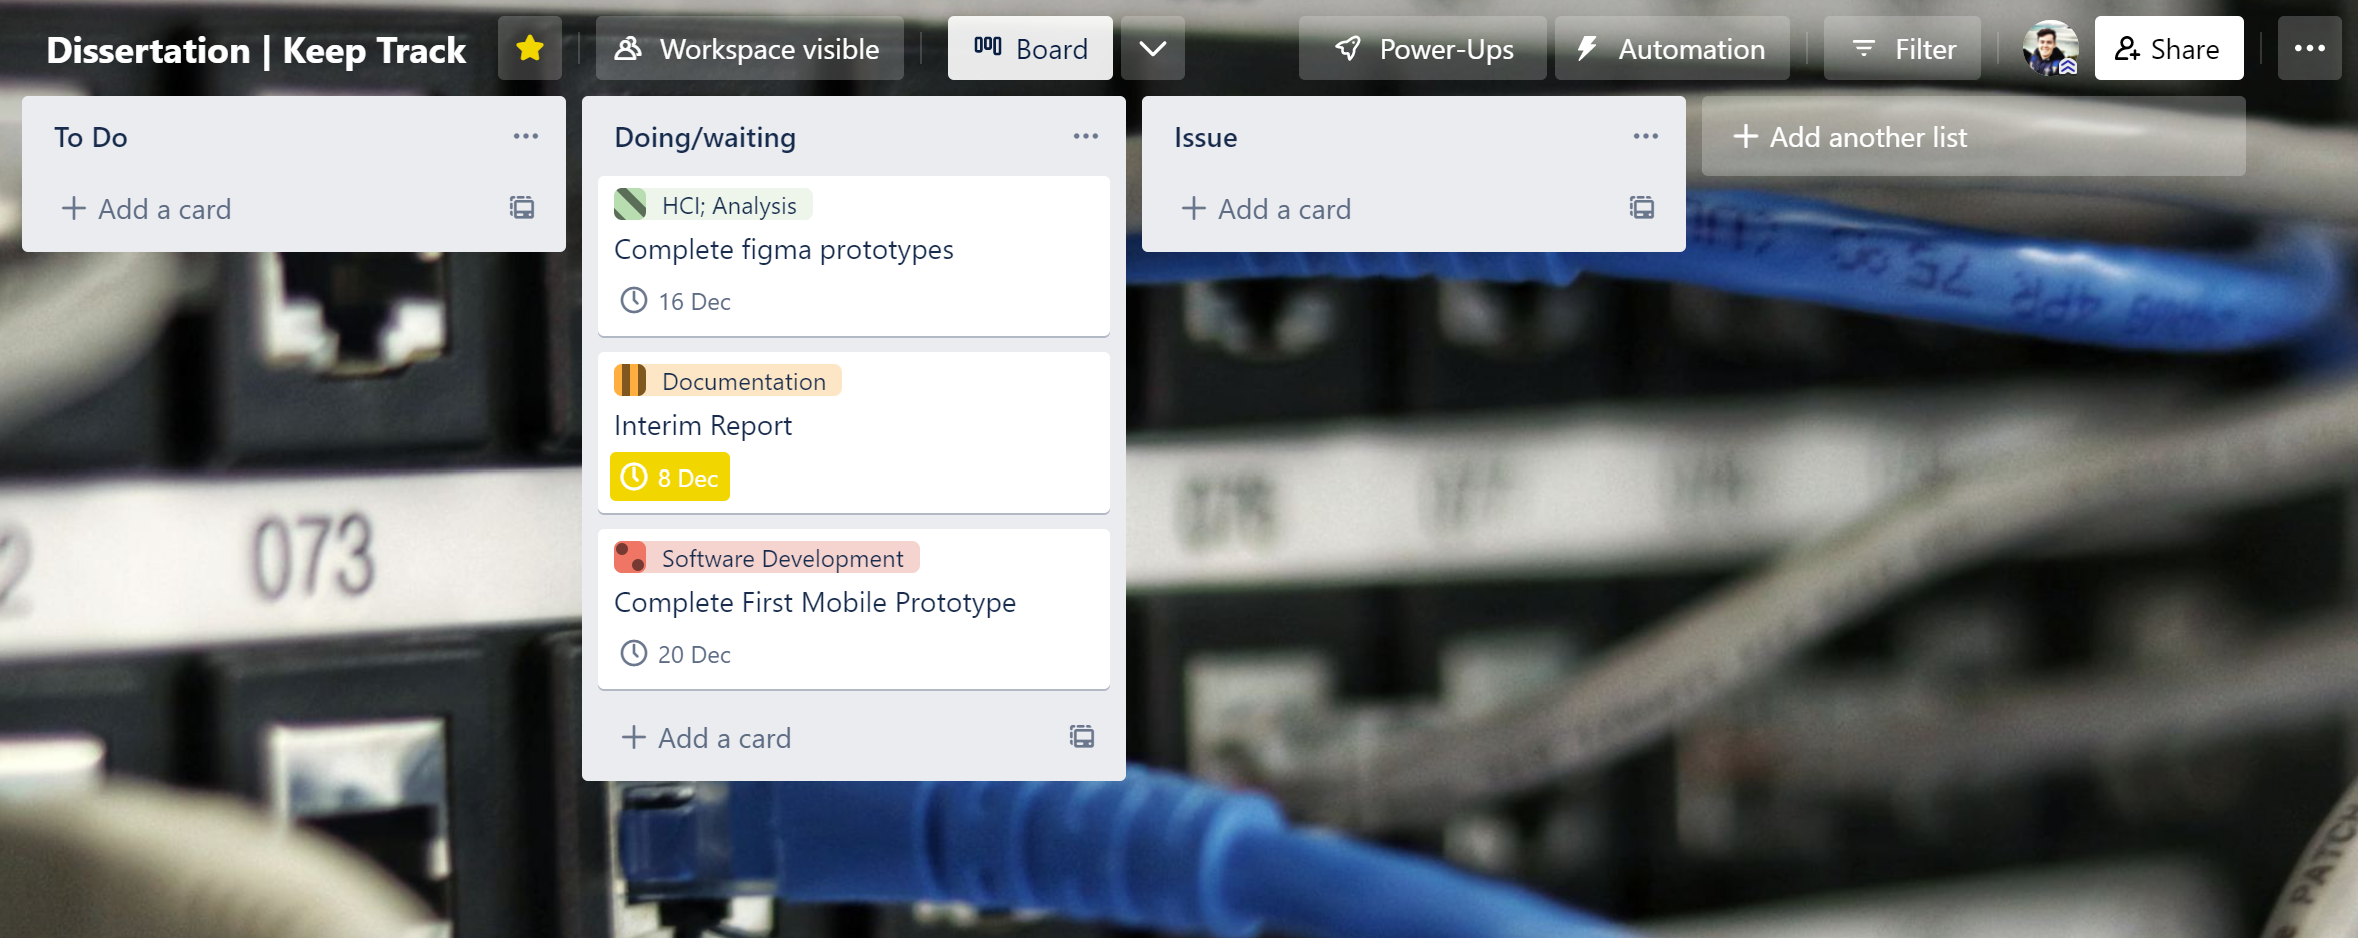
\includegraphics[width=1\textwidth]{images/trello-board.png}
\end{figure}   

\section{Initial Gantt Chart}
\label{sec:init_gantt_charts}
\begin{figure}[H]
    \centering
    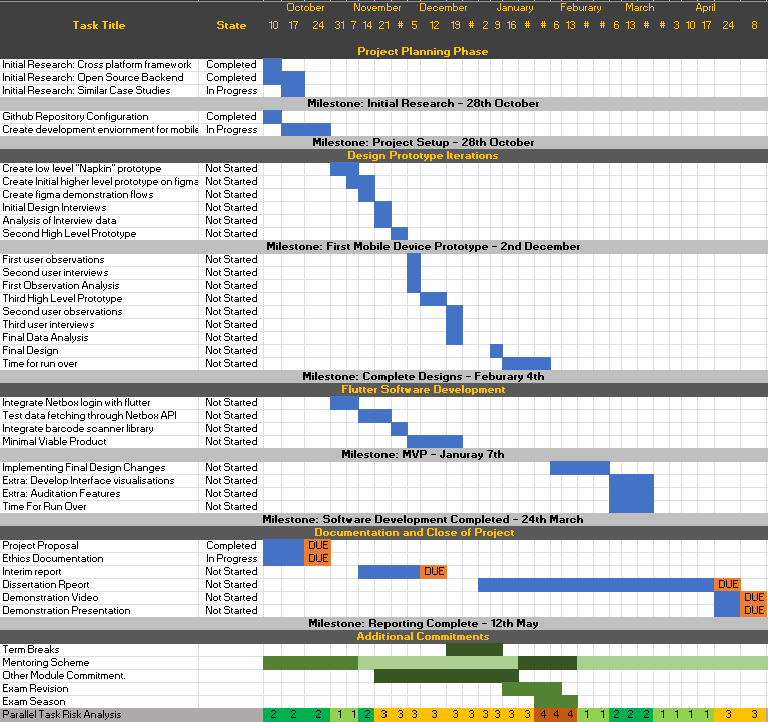
\includegraphics[width=1\textwidth]{images/keeptrack-gantt-initial.png}
\end{figure}

\section{Updated Gantt Chart}
\label{sec:updated_gantt_charts}
\begin{figure}[H]
    \centering
    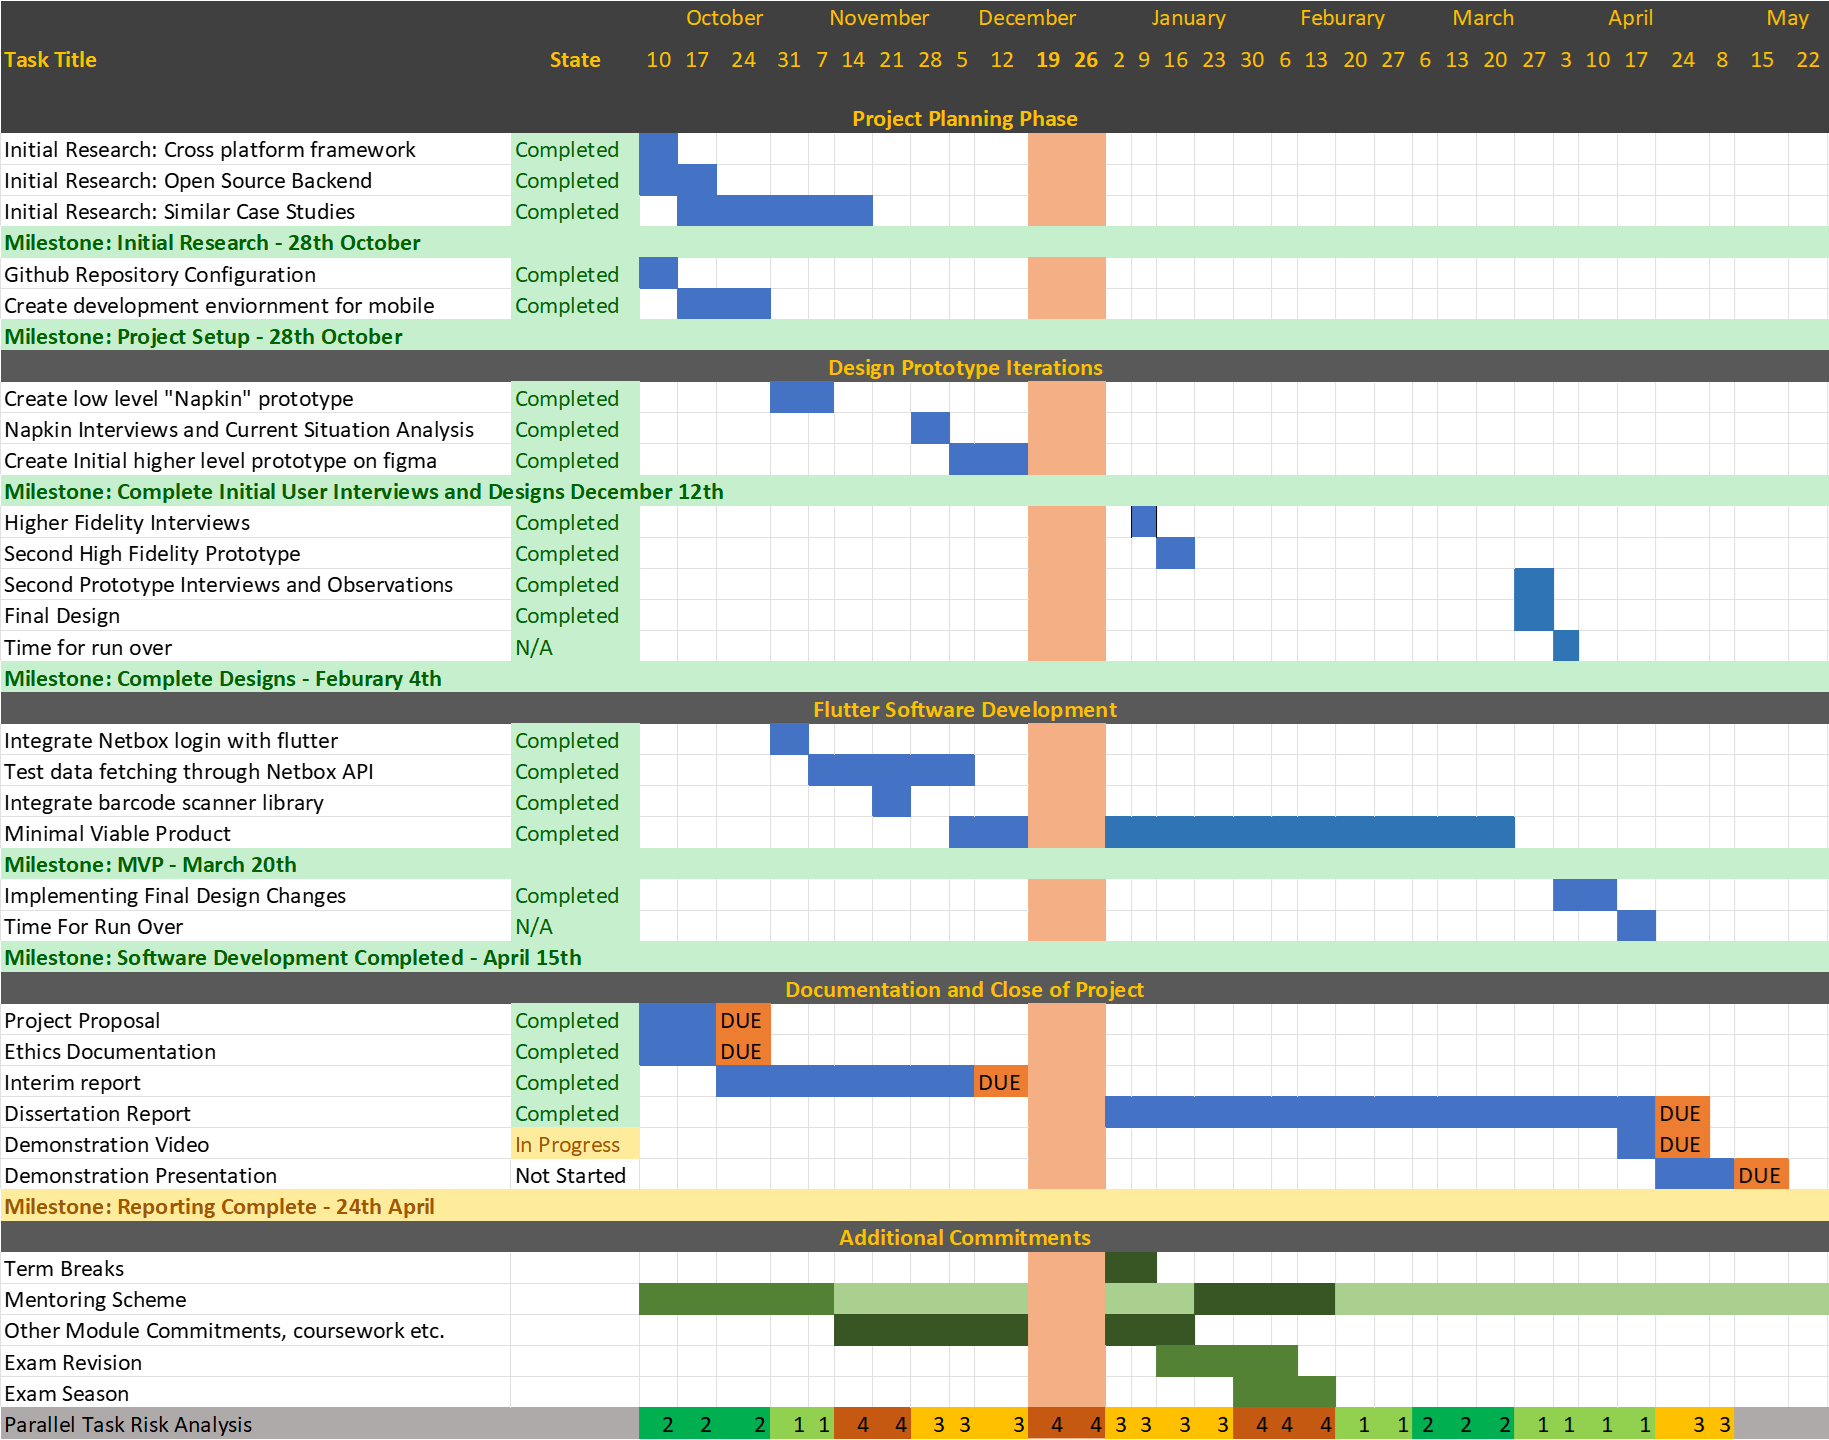
\includegraphics[width=1\textwidth]{images/keeptrack-gantt-final.png}
\end{figure}

\section{Current State Interview Insights}
\label{sec:current_state_interview_takeaways}
\subsection{Interview 1}
\label {sec:thematicAnalysisInterview1}
\begin{enumerate}  
    \item Many systems in the workplace are in "legacy mode".
    \item There is a knowledge gap due to the pandemic and staff being moved around.
    \item Documentation is lacking and not helpful in troubleshooting.
    \item When things go wrong, it takes a lot of time to diagnose and fix them.
    \item There is a reliance on poorly documented "clever solutions".
    \item There needs to be more flexibility and adaptability in the workplace.
    \item There are many outdated servers that need to be replaced.
    \item There is a lot of work to do in terms of reorganizing and replatforming systems.
    \item There are multiple single point failures in the workplace.
    \item There are unique challenges in balancing outdated and modern technology.
    \item Third parties want to assess the data centre to see if it can be integrated into a larger facility. The school is hesitant about this because they want to maintain their current system and way of working.
    \item Staff members have already expressed resistance to the idea of integrating into a larger facility.
    \item Interviewee 1 is trying to get the CVL cluster into a state where it is clearly managed to the best practices
    \item Interviewee 1 and Interviewer discuss the importance of well-labelled and well-thought-out cabling and documenting.
    \item They mention the need for a dynamic system like Netbox to help with documentation.
    \item They discuss the potential of allowing students access to the server room to learn about server management.
    \item Interviewee 1 and Interviewer discuss the lack of historical data and the need for a journaling/auditing feature once they have a clean system.
    \item It would be beneficial to capture a document that outlines a system's specifications, owner, and status, as well as the Ansible config used to build it.
    \item A third party recommends killing and rebuilding virtual machines rather than upgrading them through Yum.
    \item Changes made to a system should be documented in a journal to make troubleshooting easier in the future.
    \item An inventory system for tracking physical devices (e.g., servers, switches, cables) is needed, and it should use unique identifiers for each connection.
    \item QR codes should be placed on the front and back of servers to make identifying them easier.
    \item Sockets on the back of servers are poorly annotated and need some kind of identifier.
    \item A stretch goal is to develop an AR feature for visualizing the inventory system.
    \item The project should be designed with future improvements in mind, as new people will come and go and may need to add to or modify the system.
    \item Interviewee 1 has seen AR apps for data centres, but they look awful, and the students could do something better.
    \item AI can do better than a human being in certain tasks, such as pathology.
    \item There is a need for a simple dial to show cooling capacity in the data centre.
    \item Power cables and distribution boards need to be documented and visualised.
    \item Netbox is limited in terms of adding connections and searching, and its hierarchical structure is not ideal for adding devices.
    \item Sunbird is too much for their needs.
    \item There is a need for an app to navigate the data centre, like Pathfinder Mobile, to identify which devices are plugged in and their connections.
    \item Interviewee 1 likes the hierarchical view in the master plan, especially in the rack view.
    \item The hierarchical view is useful for visual navigation and interaction in the academic context.
    \item Interviewee 1 acknowledges the importance of having accurate and up-to-date documentation of network points and devices in different rooms and locations within the building.
    \item Interviewee 1 suggests combining the hierarchical view with documenting network cabinets or comms rooms in the future.
    \item Interviewee 1 mentions the idea of using an app to capture live socket data to be able to trace back connections.
    \item Interviewee 1 suggests adding the tracing feature after Interviewer’s dissertation.
\end{enumerate}

\subsection{Interview 2}
\label {sec:thematicAnalysisInterview2}
\begin{enumerate}
    \item Interviewee 2 thinks that the current state of the server has massively improved and that the future of it is great.
    \item The lighting improvements has made a massive difference, and power distribution has been sorted out properly without tripping.
    \item Documenting and organizing the layout of cables is important, and a focus view on Netbox could be useful.
    \item Replicating the journaling features of networks on an institute level could be beneficial.
    \item End of life and warranty information should be easily accessible in an alert.
    \item QR codes could be implemented to simplify the process of adding connections to assets.
    \item The idea of scanning cables to see the trace of connections is good.
    \item Too much information on one device can be overwhelming.
    \item AR representation of the server room and its devices would be ideal.
    \item Sunbird is too expensive and has too much information.
    \item Netbox is easier to use and visually better than Sunbird.
    \item A visual representation, such as AR, is easier to relate to than data.
    \item Interviewee 2 likes the visual arrangement of Netbox and thinks it is feature-rich.
    \item Having all the information in one place is helpful.
    \item Knowing all the information beforehand is brilliant for diagnosing issues without a site visit.
    \item The app could almost tell you what was going wrong if it's DNS DHCP issue.
    \item People move rooms without telling you, so having an inventory is useful.
    \item It would be good to have a history of changes to data.
    \item The set tags that the university uses could be used for each PC asset.
    \item A third party had all the information initially before all the walls in the building moved, and he could filter it down to Mac address and data point per switch.
\end{enumerate}

\subsection{Interview 3}
\label {sec:thematicAnalysisInterview3}
\begin{enumerate}
    \item The lack of digital or physical records for devices in the server room is the biggest problem.
    \item Modifications or upgrades of the servers are difficult due to the lack of documentation, especially for cables and console panels.
    \item Sometimes it's hard to access the servers or devices, and most of them don't have a warranty anymore.
    \item The error information needs to be gathered, and it's important to have well-considered ways to present data and record it.
    \item The server room was not designed for the purpose, and it's not necessary to have a complex system or a massive software for recording data.
    \item The app needs to have an easy and human-friendly way to add information, and form applications would be helpful.
    \item Providing some basic tools like ping and console access remotely would be helpful.
    \item Safety risks need to be considered for providing wireless signal or access to VLAN, and using a proxy could be a solution.
    \item It would be interesting to simulate live sessions with a proxy, and existing solutions should be explored.
    \item Interviewee 3 suggests that only certain people should be able to access the application.
    \item Interviewee 3 proposes adding labels to devices to make it easier to locate them and scan with the same method as cables.
    \item Interviewee 3 suggests improving the process of adding a connection by allowing users to scan device A, scan device B, and choose the interface.
    \item Interviewee 3 agrees that a view connection feature that allows users to scan the cable and search by device would be helpful.
    \item Interviewee 3 suggests that a network topology feature would be useful for viewing the entire topology of the room.
    \item Interviewee 3 states that adding one interface at a time is fine for normal servers but suggests adding an option to create multiple interfaces in bulk for devices like switches.
    \item Interviewee 3 recommends simplifying the process of showing devices by just scanning the device label and including information about interface connections.
    \item There is a need to include information about hardware settings, such as CVL, for some servers.
    \item There should be a way to view devices across different racks and filter them efficiently.
    \item Adding new devices and fields is slow and needs improvement.
    \item Interviewee 3 prefers Netbox over DC Track as it is more lightweight and less overwhelming.
    \item There is a need to add a feature for upgrading or modifying existing devices, such as changing connections.
    \item Interviewee 3 suggests adding quick links to important information, but it should be managed properly to prevent clutter.
    \item Interviewee 3 prefers to use laptop instead of mobile app for filtering and searching assets.
    \item Adding device make and model templates manually is tedious.
    \item Existing tools are not designed for mobile phones and need to be more human-readable.
    \item The viewing experience of Patch Manager on mobile is not great, but the UI looks better on the platform.
\end{enumerate}


\section{User Observations }
\label{sec:appendix_observations}
\begin{enumerate}
    \item Automatic focus of keyboard on dropdown search menus.
    \item Bug found with filtering by location on the connection search page.
    \item Arrow directions of location hierarchy are confusing.
    \item Expandable Lists for Racks with devices nested inside them.
    \item Keep the last item selected in the hierarchy when navigating back.
    \item Add more home screen buttons for quick access to common pages.
    \item Change the side menu icon to a gear icon to indicate settings.
    \item Bug with loading in interfaces on modify connection page.
    \item Add a hint to modify the connection to suggest scanning for a device or entering ID to start.
    \item Add more labels to text fields to make it easier to understand what they are for.
    \item Rename the "New Search" button to "back" and navigate one up the tree. 
    \item For interfaces that don't have a connection on them, automatically navigate the user to the Add Connection page with a click.
    \item Bug on add connection page where an error causes a white screen rather than an error message.
    \item Don't allow the user to select an interface that is already connected.
    \item Make missing fields on the add connection page more obvious - red text or highlight.
    \item The home button on the interface display isn't clear. 
    \item What interfaces the cable is connected to is not clear.
    \item Button to go from hierarchy to the device itself. 
    \item Loading interfaces indication on add and modify connection.
    \item Further work suggestion to integrate the new connection addition to a printing system.
\end{enumerate}

\end{document}